\documentclass[journal]{IEEEtran}
\usepackage[utf8]{inputenc}
\usepackage[T1]{fontenc}
\usepackage{amsmath,amssymb,amsfonts}
\usepackage{bm}
\usepackage{graphicx}
\usepackage{booktabs}
\usepackage{multirow}
\usepackage{xcolor}
\usepackage{url}
\usepackage[hidelinks]{hyperref}
\usepackage[capitalise]{cleveref}
\usepackage{placeins}
\usepackage{algorithm,algorithmic}
\newif\ifblindreview
\newcommand{\rpath}[2]{\ifblindreview#2\else\texttt{#1}\fi}
\ifdefined\BLINDREVIEW\blindreviewtrue\fi
\setcounter{topnumber}{4}
\setcounter{dbltopnumber}{2}
\renewcommand{\topfraction}{0.92}
\renewcommand{\dbltopfraction}{0.92}
\renewcommand{\textfraction}{0.08}
\renewcommand{\floatpagefraction}{0.85}
\renewcommand{\dblfloatpagefraction}{0.85}
\newcommand{\ddl}{DDL}
\newcommand{\Jobj}{J}
\newcommand{\design}{\bm{d}}
\newcommand{\soft}{\tilde{\bm{p}}}
\newcommand{\task}{\tau}
\newcommand{\E}{\mathbb{E}}
\newcommand{\Var}{\mathrm{Var}}
\DeclareMathOperator*{\argmin}{arg\,min}
\renewcommand{\thesection}{S-\Roman{section}}
\renewcommand{\thefigure}{S\arabic{figure}}
\renewcommand{\thetable}{S-\Roman{table}}
\renewcommand{\thealgorithm}{S\arabic{algorithm}}
\begin{document}
\title{Supplementary Material for ``Differentiable Design Languages: Post-Training Language-Model Design Agents with Adjoint Gradients from Physics Simulators''}
\ifblindreview
\author{Anonymous Authors}
\else
\author{Tianyu~Li, Qingang~Zhang, Hoanghuy~Nguyen, Zhiwei~Cao, Ruihang~Wang, Binyang~Song, and~Yonggang~Wen,~\IEEEmembership{Fellow,~IEEE}}
\fi
\maketitle
\ifblindreview
\markboth{IEEE Transactions on Neural Networks and Learning Systems}{Anonymous submission --- Supplementary Material}
\else
\markboth{IEEE Transactions on Neural Networks and Learning Systems}{Li \MakeLowercase{\textit{et al.}}: Differentiable Design Languages --- Supplementary Material}
\fi
This supplementary file carries thirteen sections, S-I to S-XIII.  The audits are
the estimator bias--variance audit (S-I), the non-language policy controls
(S-II), the English-constraint transfer (S-III) and the design-trajectory plate
(S-V).  The reproducibility appendix is S-IV.  The moved and extended material
is the break-even controls (S-VI), the endpoint-stability audit (S-VII), the
positioning table and post-training step (S-VIII) and the moved figures and
tables (S-IX).  The physicality audit is S-X, and the Benchmark-B post-training
tables and tests are S-XI.  Every number here is generated by the same
companion repository as the main text, and cross-references of the form
``of the main text'' point at the numbered objects of the accompanying manuscript.
\section{Bias and variance of the estimators}
\label{supp:e1}


The matched-budget race and the bias--variance table reproduce their pre-repair
values to three decimals, so the estimator comparison is robust to the benchmark
repair.
The bias--variance figure of the main manuscript (Sec.~V-C) measures, for a
single $S{=}8$-sample estimate, the cosine to the
reference gradient of $\E[\Jobj]$ and the signal-to-noise ratio
$\|\E\hat g\|/\sqrt{\operatorname{tr}\operatorname{Cov}\hat g}$.  Both are measured
over 5 tasks $\times$ 2 policy points per $N$.  With $N{=}8$ ($2N{=}16$) decisions all estimators are
poor relative to what follows: the score-function family sits at cosine $0.34$
against the pathwise family's $0.59$.  As the number of decisions grows the
score-function family degrades to $0.25$ at $N{=}16$, while the pathwise family holds
$0.57$ with $2$--$3\times$ higher SNR.  The straight-through
variant is only slightly worse than the soft one, and a higher temperature trades
cosine for SNR.  In a matched-budget optimisation race over 400 evaluations and normalised gradient
steps, the pathwise estimators drive
$\E[\Jobj]$ to $0.115\pm0.041$ ($N{=}8$) and $0.167\pm0.035$ ($N{=}16$) of its starting
value.  The race covers 5 tasks $\times$ 5 seeds per $N$, twenty-five (seed, task) cells.  REINFORCE reaches $0.231\pm0.058$ and
$0.412\pm0.047$, and GRPO $0.223\pm0.050$ and $0.402\pm0.058$.  An exact paired
signed-rank test over the cells separates pathwise from both at $p=6.0\times10^{-8}$
per $N$.  \Cref{fig:e1d} draws the race curves.  The gap widens with the number of
decisions, as the estimator statistics predict.
% source: cosine and SNR against the number of decisions from
%         ddl/case/benchA/E1c_multi/loggers/20260914T224553Z_v2/results_e1c.json (bench
%         A-v2-20260915 stamp in the same logdir) -> records[].{N,task,policy,est,cos,snr},
%         5 tasks x 2 policy points (uniform, random) x N in {4,8,16} x 7 estimators = 210
%         records; the quoted pathwise band 0.5-0.6 is mean cos of ste_t0.5 / ste_t1.0 at
%         N=8,16 (0.575 / 0.600 / 0.559 / 0.590) against reinforce / grpo 0.43 / 0.42, and
%         the 2-3x SNR claim is 0.86-1.43 against 0.42-0.51.  Matched-budget race from
%         ddl/case/benchA/E1d_race/loggers/20260916T011251Z_gpuserver/results_e1d.json ->
%         config and rows[].{N,task,seed,est,hist}; final/start of hist over the 25
%         (seed,task) cells per N gives ste_t0.5 0.1154+-0.0406 (N=8) and 0.1667+-0.0345
%         (N=16), reinforce 0.2315+-0.0575 and 0.4117+-0.0468, grpo 0.2228+-0.0504 and
%         0.4020+-0.0581 (sd ddof=1); paired exact signed-rank ste vs reinforce and vs
%         grpo p=5.96046e-08 at both N (method exact_dp, n=25 nonzero).
%         The bias/variance degeneracy records quoted in the Sec. VII preamble are the
%         sibling v2 runs of ddl/case/benchA/E1_estimators/loggers/
%         {20260915T031816Z_gpuserver (checkvalve, dT_cap 100), 20260915T031936Z_gpuserver
%         (legacy pump, dT_cap inf)}/results_e1.json -> stats[].{arm,rel_bias,rel_var};
%         that case does not produce the cos/SNR-versus-decisions curves quoted here.
%         NOT REPRODUCED from these v2 artefacts and flagged for the next pass: the
%         cosine-versus-N curve of the v1 run.  Round 9: body and figure both drawn from the v2 re-run
%         20260914T224553Z_v2; family means over tasks and policy points are
%         SF 0.366/0.338/0.247 and PW 0.448/0.588/0.568 at N=4/8/16.

The same measurement draws each fitted slope against the confidence scale at which its arm decodes, and \cref{fig:bcalib} draws it.

\begin{figure}[t]\centering
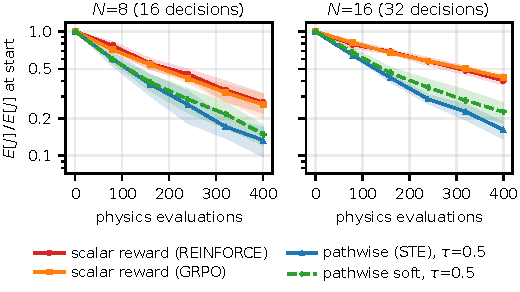
\includegraphics[width=\columnwidth]{figures/fig_e1d_race.pdf}
\caption{Expected objective, relative to its value at the uniform
policy, versus physics evaluations, for a factorised design policy trained
with each estimator ($S{=}8$ per step; 5 tasks per $N$; mean $\pm$ sd).}
\label{fig:e1d}\end{figure}


\begin{figure*}[t]\centering
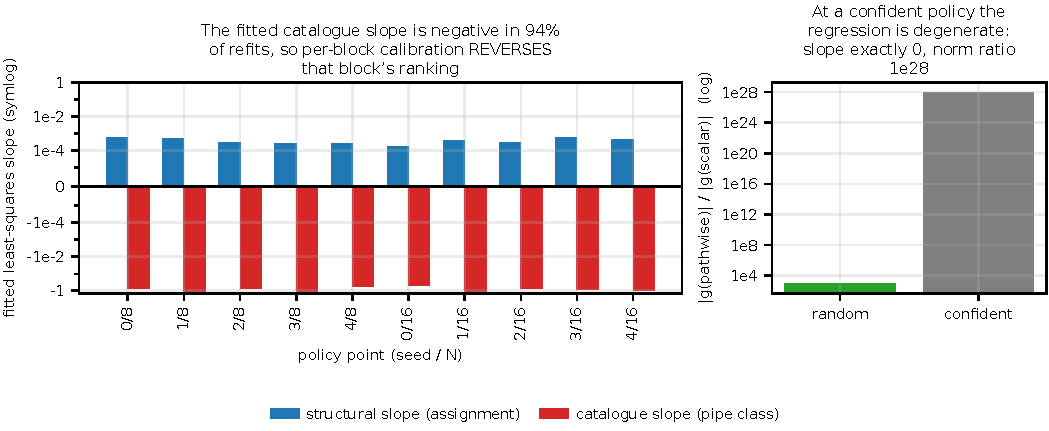
\includegraphics[width=\linewidth]{figures/fig_e1e_calib_slopes}
\caption{Why per-block affine calibration fails on the production solver, and why it fails harder the
better the policy is. \emph{Left}: the least-squares slope fitted for each decision block at 10 policy
points (5 seeds $\times$ $N\in\{8,16\}$), 24 independent refits each. The structural slope is positive and
small ($+3.80\times10^{-4}$ median) while the catalogue slope is \textbf{negative in 94\% of refits}
($-0.886$ median). Per-block calibration therefore reverses the catalogue ranking instead of rescaling it.
Under the unit-normalised step a race takes, a global scale cancels, so only this relative weighting and
the two signs survive. \emph{Right}: the pathwise-to-score-function gradient-norm ratio by policy confidence. At a
confident policy all $S$ samples decode to the same design, and the per-sample spread the slope is fitted from
collapses.  Both fitted slopes return exactly $0.0$ at a norm ratio of $10^{28}$: regression-based
calibration is undefined precisely where a converged design agent lives.}
\label{fig:bcalib}
\end{figure*}
\cref{fig:bcalib} exposes a second and more fundamental limitation:
at a \emph{confident} policy point the regression is degenerate. All $S$ samples decode to the same design, and the per-sample variance the slope is
fitted from collapses to zero.  Both fitted slopes return exactly $0.0$.  The
pathwise-to-score-function norm ratio there is $10^{28}$ for the structural block. Regression-based calibration of a pathwise estimator against a score-function
estimator is therefore \emph{undefined} precisely where a converged design agent
lives.  That is an argument against the construction itself and not only against our
parameterisation of it.
% source: ddl/case/benchB/E1e_calibration_slopes/loggers/20260914T223127Z_gpuserver/
%         results_e1e_calibration_slopes.json -> summary["random"] {a_z median
%         +3.801e-04, a_b median -8.863e-01, rho_z +0.361, rho_b -0.261,
%         frac_batches_a_b_negative 0.94, n=10 policy points x 24 refits} and
%         summary["confident"] {a_z = a_b = 0, rho = 0, norm_ratio 1.044e+28}.




\subsection{Why per-block calibration fails, and two guarded variants}
The reason calibration fails is now measured rather than asserted.  Refitting
the slope on each of 24 independent batches over ten policy points, the fitted
catalogue slope has median $-0.886$ and is negative in $94\%$ of batches,
against $+3.80\times10^{-4}$ for the structural block.  Per-block calibration
therefore \emph{reverses} the catalogue ranking instead of rescaling it, as
Supplementary Fig.~S2 shows.  Two guarded variants repair that.  A single slope for
the whole vector reaches $0.454\pm0.182$ on the relaxed objective at $N=8$,
where the pathwise arm is lower at $0.417\pm0.176$.  A per-block slope shrunk
toward norm matching and clipped at zero reaches $0.665\pm0.067$ at $N=16$, the
lowest variance in the comparison, where the pathwise arm is again lower at
$0.642\pm0.204$. It also recovers edit-selection $\rho$ from $-0.113$ to
$+0.401$.  At a confident policy point both slopes are exactly $0.0$ and the
pathwise-to-score-function norm ratio is $10^{28}$, so regression-based
calibration is undefined precisely where a converged design agent lives.
% source: relaxed-objective ratios from
%         ddl/case/benchB/E1b_estimator_types/loggers/20260915T150205Z_race5seed_calibbugfix/
%         results_e1b_lc.json -> summary.race["N8|calib_global"] 0.45403+-0.16314 and
%         ["N16|calib_shrunk"] 0.66453+-0.06002 against ["N8|ste"] 0.41719+-0.15781 and
%         ["N16|ste"] 0.64221+-0.18288 (n = 5; calib_shrunk has the lowest N16 sd of the
%         nine arms).  The superseded values 0.433 and 0.635+-0.032 came from the
%         pre-repair calibration implementation, superseded by the calibbugfix run.

\section{Non-language policy controls}
\label{supp:policies}

\emph{The 6{,}599-parameter factorised policy.}  A factorised policy reading
engineered per-rack physical features was post-trained with the same estimators and
the same \textbf{five} seeds, for 100 steps on a $2{,}000$-step supervised warm
start. The language model ran 200 steps on a 120-step warm start.  It reaches $15.73\pm9.75$ / $9.47\pm8.59$ / $7.86\pm6.63$ at a
training budget of $1{,}600$ forward solves, against $1.08$ / $4.16$ / $7.47$ for the
4B warm start.  Every $\pm$ in this subsection is the sd over seeds with the sample
divisor (ddof=1).  The graph policy trains for 2{,}000 steps on the same
$2{,}000$-step warm start; ratios across policy classes are illustrative rather than
budget-matched.  The language model is
$14.5\times$ better in distribution on validation and $2.3\times$ better on test.
Out of distribution it is not separable from the small policy at five seeds, where
the small policy's own spread ($\pm6.63$ on a mean of $7.86$) is larger than the
difference between the two.
In distribution the gap is a hypothesis-class gap rather than a budget gap: giving
the small policy $15\times$ more physics ($1{,}600\to24{,}000$ solves) leaves
validation plateaus at $11.7$--$15.6$.  Out of distribution the same budgets give
$1.68\to11.33\to0.31$ at two seeds.  That sequence is not monotone, and its endpoint
we do not claim.  This control supports no out-of-distribution ordering above.  At five seeds no paired ordering between the two policies
is claimable.  The exact signed-rank floor at $n=5$ is $p=0.0625$, which never reaches
$\alpha=0.05$ at any effect size.  Six seeds is the smallest count that can.  What
survives is the plateau itself, i.e.\ that the
in-distribution gap is a hypothesis-class gap rather than a budget gap. The estimator ordering inside this control is the cleanest evidence in the paper
for the mechanism itself. One caveat: the score-function arms of this control
carry no reward transform and diverge at every point of a six-point learning-rate
sweep. The ratios measure the divergence of an untransformed baseline rather than
estimator quality; the mechanism evidence rests on the within-invocation
graph-versus-factorised contrast and on the language-model arms.  Pathwise beats
score-function by $169\times$ on validation
regret ($15.73\pm9.75$ against $2665.10\pm558.03$), by $298\times$ on test
($9.47\pm8.59$ against $2818.52\pm617.36$) and by $349\times$ out of distribution
($7.86\pm6.63$ against $2742.96\pm615.07$).  The out-of-distribution ratio is not
separately significant.  All three hold at a comparable budget, on a CPU, in
$9.5$\,s.  The score-function arms do not merely fail to improve: they destroy the shared warm
start.  On validation it goes $21.5\to2665.1$, feasibility is exactly $0.00$, and the
Hamming distance to the reference equals the full slot count on all three splits.  They
collapse to one deterministic infeasible design.
% source: ddl/case/policy/small_policy_posttrain/loggers/20260915T150017Z_matched5/
%         results_small_policy.json (config.seeds = 5, n_params 6599, bench A-v2-20260915,
%         checkvalve / dT_cap 100) -> summary["ste|{val,test,ood}"]
%         {regret_median_mean 15.7251 / 9.4654 / 7.8595, regret_median_all giving ddof=1 sd
%         9.75 / 8.59 / 6.63, total_solves 1600 forward, wall_secs 10.5} and
%         summary["reinforce|{val,test,ood}"].regret_median_mean 2665.10 / 2818.52 / 2742.96
%         (ddof=1 sd 558.03 / 617.36 / 615.07).  The 169x / 298x / 349x are those pairs
%         split by split; no paired test between them is archived, hence "not separately
%         significant".  4B warm start 1.08 / 4.16 / 7.47:
%         ddl/case/analysis/v2A_table/loggers/20260915T163846Z_gpuserver/
%         results_v2A_table.json -> warm_start.{val,test,ood}.regret_median.  Budget
%         plateau (1,600 -> 24,000 solves) and the two-seed ood sequence:
%         loggers/sweep_20260914T195608Z_gpuserver.  Run 20260915T004012Z_matched3
%         (config.seeds = 3) is superseded for every number in this control.
%         ddl/docs/FINDINGS_2026-09-15.md Sec. 13.

\emph{The 16{,}260-parameter graph policy: the hypothesis class is the variable
that mattered.}  The factorised control reads engineered per-rack features.  It cannot
see that two racks in one corridor compete for the same coolant path. A bipartite rack/corridor graph policy with a two-layer pair head was post-trained
in the same process from the same shared warm start, with the same estimators, the
same budget and \textbf{five} seeds.  It reaches $2.25\pm1.66$ / $0.68\pm0.77$ / $1.09\pm0.69$ against the factorised
policy's $13.33\pm6.09$ / $5.74\pm3.47$ / $6.77\pm4.28$ within the same pinned
invocation: $5.92\times$ / $8.41\times$ / $6.20\times$, with exact paired Wilcoxon
$p=0.0035$ / $8.0\times10^{-5}$ / $0.014$.  Against the five-seed factorised runs of a
separate invocation ($15.73\pm9.75$ / $9.47\pm8.59$ / $7.86\pm6.63$) the ratios are
$6.98\times$ / $13.88\times$ / $7.21\times$; the within-invocation values are primary
because the repository's ratio rule forbids crossing invocations.  The
pairing is significant on all three splits.  Every graph-policy number above comes
from an invocation pinned to a single thread, because the policy's aggregation is a
float reduction whose order depends on the thread count. Four pinned invocations
reproduce all eighteen summary cells bit-identically, while unpinned invocations
disagree in nine of eighteen.  Against the
same statistic the five-seed language-model arm of Table~I of the main text records $0.57$ /
$0.32$ / $0.27$. The ordering language model, graph policy, factorised policy
holds within one statistic on all three splits.
% source: the factorised triple is the control's own five-seed run,
%         ddl/case/policy/small_policy_posttrain/loggers/20260915T150017Z_matched5/
%         results_small_policy.json -> summary["ste|{val,test,ood}"].regret_median_mean
%         15.73 / 9.47 / 7.86; that is the single triple this paper uses for the
%         6,599-parameter policy; the 13.33 / 5.74 / 6.77 triple is the in-process
%         factorised arm of the same pinned invocation and is quoted only as such.  Graph-policy triple from
%         ddl/case/policy/GNN_baseline/loggers/20260915T150746Z_gpuserver_pin1/
%         results_gnn_policy.json -> summary["gnn_ste|{val,test,ood}"]
%         {regret_median_mean 2.2514 / 0.6818 / 1.0908, regret_median_sd_sample
%         1.6613 / 0.7652 / 0.6942}.  The 6.98x / 13.88x / 7.21x are those two triples
%         divided split by split.  The Wilcoxon and McNemar p-values beside them are the
%         SAME-PROCESS contrast archived in that pinned run,
%         tests.contrasts[arm_a=gnn_ste, arm_b=mlp_ste] (val 0.0034715, test 7.9968e-05,
%         ood 0.014046; McNemar 0.00031075 / 0.00091052 / 0.189247), where the factorised
%         comparator was retrained inside the invocation and is
%         summary["mlp_ste|{val,test,ood}"].  Re-deriving those paired tests across the
%         two invocations is outstanding with the p-value regeneration pass.  Language-model
%         medians 0.57 / 0.32 / 0.27:
%         ddl/case/analysis/v2A_table/loggers/20260915T163846Z_gpuserver/
%         results_v2A_table.json -> table.ste.{val,test,ood}.mean_of_medians
%         0.5714 / 0.3200 / 0.2672; the superseded 0.58 / 0.57 / 0.26 matched no key.
Its first version underfit badly, at training cross-entropy $1.30$--$1.82$ against
the factorised policy's $0.995$.  Its pair score was a single linear map and so
additive in the two node states, unable to express a rack$\times$corridor
interaction.  The two-layer head gives $0.6150$.  Exact McNemar
on feasibility gives $p=0.00031$ ($23$ tasks gained, $4$ lost) and $0.00091$ ($21$
gained, $4$ lost) in distribution and on test, and $p=0.19$ out of distribution ($14$
gained, $7$ lost).  The $24$-configuration screen behind it is archived and
selected on \emph{training} cross-entropy and then training Hamming distance, never on the comparison metric. The regret ratios above compare the two policies across independent runs, while
the feasibility McNemar and the regret Wilcoxon compare them within the same pinned
process; the two comparisons are deliberately not mixed.

Two properties of this control matter more than the ratio. Its \emph{zero-physics} floor is statistically indistinguishable from the
factorised policy's \emph{post-trained} arm on all three splits ($p=0.47$ / $0.95$ /
$0.71$).  The $1{,}600$ forward solves that the factorised policy spends therefore buy nothing this warm start
does not already have. And against the language model's warm start ($1.08$ / $4.16$ / $7.47$, at zero
physics) it is $2.07\times$ \emph{worse} in distribution but $6.10\times$ better on
test and $6.85\times$ better out of distribution.  That \emph{reverses} the ordering
the factorised policy reports.  That reversal is provisional:
 it compares a post-trained policy against its own warm start, while the matched
five-seed language-model comparison lives in Table~I of the main text under the median statistic. The defensible statement is
narrower and more useful --- no ordering between a language model and a non-language
policy survives a change of hypothesis class --- and the abstract is scoped to say that.
% source: ddl/case/policy/GNN_baseline/loggers/20260915T150746Z_gpuserver_pin1/
%         (authoritative pinned logger; the unpinned loggers agree)
%         results_gnn_policy.json -> summary and tests.contrasts (the tests are IN the
%         artefact now, round-4 N-9), policies.{gnn,mlp}.n_params 16260/6599, config
%         {seeds 5, arms sft/ste/reinforce, sft_steps 2000, threads 1}, torch_num_threads 1,
%         bench A-v2-20260915, bench_config {checkvalve, 100.0}. One invocation, both policy
%         classes in the same process, ddof=1. Screen: loggers/screen_20260915T022500Z_gpuserver.
%         REPRODUCIBILITY, and why this invocation and not the earlier one: the RackGNN
%         aggregates over incident racks and corridors, a float reduction whose ORDER depends
%         on the thread count, and 2000+100 steps amplify it -- a re-run of the earlier
%         invocation at an identical config moved nine of eighteen summary cells (gnn_ste|test
%         1.5718 -> 0.3303, Wilcoxon ood 0.083 -> 0.265) while all nine RackPolicy cells
%         reproduced to +0.0000. The case now pins --threads (default 1) and stamps
%         torch_num_threads and torch_version into the JSON; four pinned threads=1
%         invocations agree on 18 of 18 cells and 9 of 9 contrasts, unpinned ones differ
%         in 9 of 18 (analysis/consistency_inputs f_gnn_spread). Invocations
%         20260915T023242Z and 20260915T072617Z are SUPERSEDED for every gnn_* number; their
%         mlp_* cells still reproduce and row P3 is RackPolicy only. FINDINGS s33.
%         Bootstrap percentile bounds are ORDER-DEPENDENT (bootstrap_ci draws index arrays and
%         takes the median over them): the val bound is [-6.4002,+0.0000] seed-major against
%         [-5.6573,+0.0000] task-major, and test/ood are identical under both. Any quoted
%         interval must name its pairing order; Wilcoxon and McNemar are order-invariant.

\emph{(e) The non-learned references, and what a regret number is worth.}  Seven
arms that learn nothing run on the same $40$ evaluation rows; five are reported here
and the nearest-greedy and underfit-head arms are archived with them.  The two stochastic ones
use five draw seeds and are reported as mean $\pm$ sd over those five draw seeds. Uniform random over the design space gives $296.03\pm135.41$ /
$511.53\pm190.18$ / $565.91\pm153.92$ at feasibility $0.050$ / $0.013$ / $0.000$ for one
solve. Drawing until a design is \emph{legal} gives $1.41\pm1.10$ / $4.38\pm3.86$ /
$23.39\pm11.22$ for $1$--$32$ solves at feasibility $0.463$ / $0.338$ / $0.075$.  That
is \emph{not} better than the language model's warm start in distribution ($1.08$) on
aggregate: it is better on $3$ of the $5$ draw seeds and worse on $2$.  A per-seed
range of $0.75$ to $3.35$ straddles the warm start.  The five deterministic arms are unaffected and
reproduce exactly. A single-step adjoint-guided greedy ranks the candidate edits by the adjoint's
predicted $\Delta\Jobj$, applies the best of three probed edits, and repeats.  It
reaches $0.153$ / $0.097$ / $0.076$ at feasibility $0.69$ / $0.63$ / $0.75$, for
$9.0$--$12.5$ forward plus $2.0$--$2.9$ adjoint solves \emph{per task}.  That is
$7.1\times$ / $42.9\times$ / $98.1\times$ better than that warm start and $126\times$
/ $97.6\times$ / $103.4\times$ better than the factorised policy. Scoring the stored
labels as designs gives exactly $0.0000$ at feasibility $1.000$ on all three splits, which
is the verification that the labels \emph{are} the best-known reference of
Sec.~VI-A of the main text. An alternating master/subproblem decomposition, not a cut-based Benders scheme,
reaches $0.0242$ / $0.0169$ / $0.0385$ for $514$--$1{,}111$ forward solves.  It
attains the proven optimum exactly on $8$ of the $12$ enumerable rows, being at most
$10.67$ above it on the other four.

The honest reading is that a twelve-solve adjoint-guided greedy beats every learned
designer in this paper, so the contribution here is not a better single-task designer. It
is the measurement of when the gradient can be trusted at all. The same adjoint used to \emph{prune} the neighbourhood instead of to rank it gives
feasibility $0.19$ at the exact-adjoint top-1 pruning against the top-8 on
validation.  That is the operational form of the decision-type asymmetry of
Sec.~VII-B of the main text, measured in the inference-search case of the accompanying
repository.  The greedy above
spends about twelve solves per task precisely because it does not trust a first-order
prediction beyond the one edit it verifies.
% source: ddl/case/policy/greedy_and_oracle/loggers/20260915T092629Z_gpuserver/
%         results_greedy_oracle.json -> summary[<arm>|<split>].{regret_median,feasible_rate},
%         rows[].physics, rows[].regret_vs_true, config {seeds 5, rand_draws 32, max_enum 8000},
%         bench A-v2-20260915. All 15 of this case's log.jsonl files carry a done row.
%         N-7: 0.0000 against the proven optimum is a MEDIAN over the 12 enumerable rows and
%         not a per-row universal. rows[].regret_vs_true is exactly 0.0 in 8 of 12 for
%         alternating_decomp (max +10.6723) and non-zero in 9 of 12 for sensitivity_greedy
%         (max +18.6234) against medians 0.0584 / 0.0770, which is why the body quotes
%         medians and claims no universal.

Taken together these five controls say something more specific than "the language
model is unnecessary" and something less comfortable than "it works". The mechanism
this paper is about --- routing a differentiable solver's gradient into an amortised
design policy --- is demonstrated most sharply by a $6{,}599$-parameter model on a
CPU. The language model's advantage is concentrated in \emph{fitting the task-to-design
mapping in distribution}.  On unseen scale the two are not separable at five seeds.
No claim about generalisation to larger $N$ is therefore available to either side. The comparison that matters is therefore not text versus weights but \emph{who
consumes the gradient}.  A search loop may consume it one edit at a time, a model may
consume it as text, or a model whose weights were updated by it may consume zero
physics evaluations per task.
These are not interchangeable, and the ordering is a property of how the
linearisation is consumed rather than of how much information was supplied. Any claim that a \emph{language} model is required must rest on what a factorised
policy over engineered features structurally cannot express: constraints stated in
natural language, and task families whose features were never engineered.  That is
what the out-of-distribution case has to probe. Larger $N$ alone is not that axis: at five seeds the language model and the
factorised policy are tied there.  A change in sequence length is in any case the
wrong probe for a claim about language, because it confounds the interface with the
length the decoder was trained on.


\section{Transfer to constraints stated in English}
\label{supp:e4text}


The three controls above bound what post-training buys on the objective the agent was trained on. They leave one question open, and it is the only question on which a
\emph{language} model is the sole candidate.  Can the agent honour a constraint that
was never a training target and was never engineered as a feature? A factorised policy over local physical features cannot express ``racks R1 and R2 must share a
CDU'' without being retrained with that feature, and an unconstrained search cannot express it at all.

Seven constraint families are generated with exact machine-checkable predicates
over the decoded design, so satisfaction is never judged by reading model output.
They are: shared CDU, distinct CDUs, forbidden CDU, a cap on how many racks one CDU
may serve, and a cap on how many racks may use one pipe class.  The last two are a
group that must share a pipe class, and a minimum number of distinct pipe classes. Each task is tested on three draws of
\emph{two} constraints at once; no training row contains any of these strings. Two arms cannot see the constraint and serve as the chance reference: the
$6{,}599$-parameter policy of Sec.~VII-G of the main text (third control), loading the same trained weights,
and an unconstrained search.  One further arm sees the constraint as a hard predicate
on candidate edits, which is the strong reference. That reference is made strong
deliberately: edits are ranked lexicographically by (violates, predicted $\Delta\Jobj$) rather than
filtered, because the fixed starting design may already violate the constraint and a filter could then
never repair it. Filtering scores $0.500$; the lexicographic search scores $0.825$. An arm that beats a
weak reference has shown nothing.  \Cref{fig:e4text} draws the per-cluster follow
rates of this comparison.

\begin{figure}[t]\centering
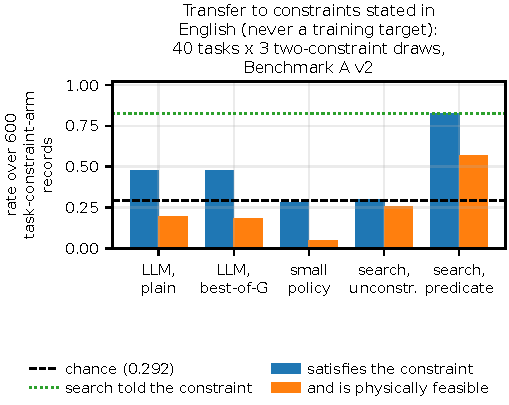
\includegraphics[width=\linewidth]{figures/fig_e4_text_constraints}
\caption{Transfer to constraints stated in English, over 600 task-constraint-arm records (40 tasks
$\times$ 3 two-constraint draws $\times$ 5 arms). Dark bars: the arm's decoded design satisfies the
constraint. Light bars: it satisfies the constraint \emph{and} is physically feasible --- the joint rate,
which is the one that matters, since a legal but unsimulatable design is not a design. The dashed line is
chance, the mean of the two arms that cannot see the constraint at all ($0.292$); the dotted line is a
search handed the same constraint as a hard predicate ($0.825$). The frozen base reaches $0.725$ at one
physics evaluation and the supervised warm start $0.475$; imitation training on design labels costs
$25$ points of compliance.  The $6{,}599$-parameter policy sits at $0.283$, indistinguishable from
chance exactly as its hypothesis class predicts.}
\label{fig:e4text}
\end{figure}
Over $40$ tasks $\times$ $3$ draws, \cref{tab:e4} reports satisfaction and quality
separately:

\begin{table*}[t]\centering\caption{Transfer to held-out ``textual'' constraints, Benchmark~A v2, 40
tasks $\times$ 3 two-constraint draws. ``Both'' is the joint rate: satisfies the constraint ``and''
physically feasible. Regret$|$both is the median regret restricted to tasks where the arm achieved both,
so it measures design quality ``under'' the constraint rather than trading it off against compliance.
The graph policy and the unconstrained search cannot see the constraint and are the chance references}
\label{tab:e4}
\fontsize{7.2}{8.4}\selectfont
\begin{tabular}{@{}lccccc@{}}\toprule
arm & satisfies & feasible & both & regret (med.) & regret$|$both \\
\midrule
\multicolumn{6}{@{}l}{\emph{v2 supervised warm start}}\\
\texttt{LLM, plain prompt} (1 solve) & 0.475 & 0.292 & 0.192 & 4.902 & \textbf{0.0785} \\
\texttt{LLM, best-of-G} (8 solves) & 0.475 & 0.292 & 0.183 & 4.874 & 0.0764 \\
graph policy (1 solve) & 0.283 & 0.225 & 0.050 & 8.932 & 0.2707 \\
\texttt{search, unconstrained} (81) & 0.300 & 0.775 & 0.258 & \textbf{0.0999} & 0.0308 \\
\texttt{search, predicate} (68) & \textbf{0.825} & 0.683 & \textbf{0.567} & 0.1899 & 0.1248 \\
\midrule
\multicolumn{6}{@{}l}{\emph{frozen base, no adapter}}\\
\texttt{LLM, plain prompt} (1 solve) & \textbf{0.725} & 0.283 & 0.192 & 11.220 & 0.3871 \\
\texttt{LLM, best-of-G} (8 solves) & 0.717 & 0.300 & 0.217 & 8.891 & 0.3753 \\
\bottomrule\end{tabular}\end{table*}

\cref{tab:e4} gives the per-arm satisfaction, feasibility and joint rates behind
\cref{fig:e4text}.
% source: ddl/case/llm/E4_ood_transfer/loggers/20260914T225146Z_warmstart and
%         20260914T225146Z_frozenbase -> results_e4_text_constraints.json,
%         summary[<arm>].overall {satisfied_rate, feasible_rate, both_rate, regret_median,
%         regret_median_satisfying, physics_mean}; 600 records per condition.
%         chance level = mean(small_policy 0.283, search_uncon 0.300) = 0.292.

Four things follow.

\emph{The language interface does something no other interface can.} Chance is $0.292$. The frozen base
reaches $0.725$ ($+43.3$ points) and the warm start $0.475$ ($+18.3$ points), at \textbf{one} physics
evaluation. The factorised policy, trained on the same labels, sits at $0.283$ --- indistinguishable from
chance, exactly as its hypothesis class predicts. This is the only measurement we
have that a language model contributes something a smaller model structurally cannot.
% P1-k: the control loaded here is case/policy/small_policy_posttrain/loggers/
%       20260914T224933Z_ckpt/policy_ste_s0.pt -- ONE seed, val 18.40 / test 14.80 / ood 1.33
%       (row P12).  The "regret of 15.6" this sentence used to carry is the TWO-seed scaling run and
%       Sec. VII-F(c) reports the THREE-seed matched3 run (19.27+-6.00), so the number was deleted
%       rather than moved: three invocations, none of them the one whose weights are loaded.
%       Re-running this arm from a matched3 checkpoint is the clean fix and is outstanding.

\emph{And the effect now survives a test that respects its grouping}.  The case
archives all $600$ per-draw records ($5$ arms $\times$ $40$ tasks $\times$ $3$
constraint draws) with the constraint index and the task seed, so an exact test is computable.  Because three draws come from one task, the primary test swaps the two
arms \emph{within} task over $40$ clusters.  An unclustered exact McNemar on the same
$120$ rows is reported beside it; it is anti-conservative in the way
Sec.~VII-D of the main text already records for a pooled count. For the \textbf{frozen base} the advantage over the factorised policy is
significant on validation ($+0.542$, permutation $p=0.0003$) and on test ($+0.375$,
$p=0.0042$).  It is \emph{not} significant out of distribution under the primary test
($+0.375$, Monte-Carlo permutation $p=0.064$ over $8$ clusters, $2\times10^{5}$ draws).  There only the
task-resampled interval $[+0.125,+0.583]$ excludes zero.
The artefact's own rule is that the clustered test governs when the two disagree, so the honest count is
two splits of three, on the weakest interval in the paper.  Against the \emph{other} blind
arm the verdict differs: the unconstrained search is now split-resolved too, and there the
frozen base is significant on all three splits ($+0.479$ at $p=0.00087$, $+0.354$ at
$p=0.0036$, $+0.458$ at $p=0.0398$).  So the out-of-distribution verdict is comparator-dependent: significant against a
search, not significant against a factorised policy.  At $8$ clusters, of which $7$ carry a nonzero
difference, the exact enumeration floor is $0.0156$ and the enumerated two-sided
$p$ is $0.0625$ (the archived Monte-Carlo estimate is $0.0637$ at $2\times10^{5}$
draws). This split therefore cannot reach $0.05$. A sibling invocation whose floors were
computed over pairs rather than clusters is superseded by this one.  ``Every
interface that cannot read it'' is therefore still not established by a single test. For the \textbf{warm start} the pooled effect is significant ($+0.183$ over chance,
interval $[+0.075,+0.292]$; $+0.192$ over the factorised policy, $p=0.016$, interval
$[+0.050,+0.333]$).  It is nonetheless \emph{entirely a validation effect}: on test
the difference is $+0.083$ at $p=0.64$ and out of distribution $+0.042$ at $p=1.00$,
both intervals spanning zero. The alignment tax below is therefore not only a $25$-point level shift: it removes
the significance of the effect on the two held-out splits.  The defensible form of the
claim is that the \emph{untrained} model satisfies an English constraint significantly
better than any interface that cannot read it.  The imitation-trained one does so
only where it was trained. Two limitations travel with this.  One model seed means the clustered test
addresses task grouping and not weight-initialisation variance, which Sec.~VII-D of the main text establishes is real, since the trainer is not run-to-run deterministic.  The control
policy is the single-seed checkpoint noted above.
% source: ddl/case/analysis/e4_significance/loggers/20260915T072042Z_gpuserver/
%         results_e4_significance.json -> comparisons[] {condition, split, difference,
%         cluster_permutation.p, cluster_bootstrap.{ci_low,ci_high}, mcnemar_exact_unclustered}
%         and verdict.txt.  Every published rate was re-derived from the E4 artefact before any test
%         was run on it (reproduction block: 0.475 / 0.2833 / 0.300 / 0.825 / 0.725 / 0.7167 all
%         match to <5e-4).  Primitives are imported from ddl/tools/summarize_runs.py, not reimplemented.

\emph{Imitation training on design labels costs instruction-following.}  The frozen
base satisfies $0.725$; after the supervised warm start the same architecture
satisfies $0.475$, a $25$-point drop.  Its unconstrained design quality meanwhile
improves from regret $11.22$ to $4.90$. That is an alignment tax, measured, on precisely the axis this paper claims is the
language model's reason to exist.  It means the post-training story cannot be told as
monotone improvement, because nothing in the objective rewards constraint compliance.

\emph{A search given the constraint as a predicate beats a model given it in
English}: $0.825$ against $0.475$ on satisfaction and $0.567$ against $0.192$ on the
joint rate, for $68$ solves against $1$.  The gap is significant at $40$ clusters
($p<10^{-4}$, interval $[-0.450,-0.250]$). Against the \emph{frozen} base the same search is ahead by only $0.100$, which is
not significant ($p=0.112$, interval $[-0.208,+0.008]$).  An untuned language model
reading one sentence is statistically indistinguishable from $68$ solves of
constrained local search. Natural
language is expressive enough to state a constraint and not precise enough to enforce it. This is
Sec.~VII-G of the main text from the other direction. There, single-edit sensitivities given as text were read
but not disciplined; here, a whole constraint given as text is understood but not reliably executed.

\emph{Conditional on succeeding, the designs are good, and that is not the binding constraint.} Among tasks
where an arm both satisfies and stays feasible, \texttt{LLM, plain prompt} reaches regret $0.0785$, better than
the constrained search's $0.1248$. The failure is the \emph{joint} rate: $0.192$, so on $80.8\%$ of tasks
the model does not produce a design that is simultaneously legal and physically valid. Separately, constraints are not free.  The unconstrained search reaches regret
$0.0999$ at satisfaction $0.300$, while the constrained one reaches $0.1899$ at
$0.825$.  Honouring the requirement therefore roughly doubles the regret, which is
why satisfaction and quality are never collapsed into one number here.

What this licenses is narrow, and we state it narrowly.  A language-model design
agent can honour a structural constraint it was never trained on and that was never
engineered as a feature, at one physics evaluation.  A $6{,}599$-parameter policy
trained on the same labels sits at chance there. What it does not license is that this beats a constrained search (it is
$1.7\times$ worse on satisfaction and $2.9\times$ worse on the joint rate).  It also
does not license that post-training improves it, since the warm start is $25$ points
worse than the frozen base.  Nor that the resulting designs are usable without
checking.


\section{Reproducibility: task generation, splits and solver constants}
\label{supp:repro}

Every constant needed to rebuild either benchmark is listed here.
Each value is read from the frozen source named beside it, not restated from prose.
\ifblindreview
Benchmark~A is the synthetic solver module of the companion repository, version
\texttt{A-v2-20260915}; its tasks and splits come from the repository's agent and
data scripts and are archived as split files.  Benchmark~B is the companion
repository's liquid-cooling solver over its network generator, version
\texttt{B-lc-20260915}; its splits come from the repository's data script and are
archived likewise.
\else
Benchmark~A is \texttt{ddl/\allowbreak src/\allowbreak thnet.py}, version
\texttt{A-v2-20260915}.
Its tasks and splits come from
\texttt{ddl/\allowbreak src/\allowbreak llm/\allowbreak ddl\_agent/\allowbreak data.py}
and \texttt{ddl/\allowbreak src/\allowbreak llm/\allowbreak make\_data.py}, and are
archived in \texttt{ddl/\allowbreak src/\allowbreak llm/\allowbreak data/\allowbreak bench.json}.
Benchmark~B is \texttt{ddl/\allowbreak src/\allowbreak softlc.py} over the network builder
\texttt{ddl/\allowbreak src/\allowbreak netgen.py}, version \texttt{B-lc-20260915}.
Its splits come from \texttt{ddl/\allowbreak src/\allowbreak lc\_data.py}, and are archived in
\texttt{ddl/\allowbreak src/\allowbreak llm/\allowbreak data\_B/\allowbreak bench.json}.
\fi
Both solvers run in float64.

Both benchmarks minimise one functional form,
\begin{equation}
\begin{split}
\Jobj \;=\;& \frac{P_{\mathrm{pump}}}{100}
\;+\; \lambda_{\mathrm{cost}}\,\mathrm{cost} \\
&+\; \lambda_T \sum_i \bigl(v_{T,i} + v_{T,i}^{2}\bigr)
\;+\; \lambda_Q \sum_k \bigl(v_{Q,k} + v_{Q,k}^{2}\bigr),
\end{split}
\end{equation}
with identical weights on both: $\lambda_{\mathrm{cost}}=0.05$, $\lambda_T=20.0$,
$\lambda_Q=500.0$.
The hinge $v+v^2$ is deliberate, so that a small violation is never cheap.
What differs is the physics, the normalisation of each $v$, and the task draws.
\Cref{tab:reproA} and \cref{tab:reproB} give all three.

\begin{table*}[!t]\centering\caption{Benchmark~A (\rpath{ddl/src/thnet.py}{the companion repository's synthetic solver module}, \texttt{A-v2-20260915}): solver, task-generation and
penalty constants.  \texttt{U}(a,b) denotes one draw from the seeded
\texttt{torch.Generator} of \texttt{random\_task}; draws are independent and taken in the order
listed.  Conductances are in kg$^2$\,s$^{-2}$\,kPa$^{-1}$, so that
$\Delta p=\dot m|\dot m|/C$ is in kPa.  The design variables are the soft assignment
$z\in[0,1]^{N\times K}$ and the soft catalogue $b\in[0,1]^{N\times M}$, both row-stochastic}
\label{tab:reproA}
\fontsize{7.2}{8.4}\selectfont\setlength{\tabcolsep}{4pt}\setlength{\emergencystretch}{1em}
\begin{tabular}{@{}p{0.180\textwidth}p{0.162\textwidth}p{0.560\textwidth}@{}}\toprule
quantity & code name & value \\
\midrule
\multicolumn{3}{@{}l}{\emph{Pipe law, fluid and pump}}\\
pipe law & \texttt{pipe\_flow} & $\dot m=\sqrt{C}\,\Delta p\,/\sqrt{|\Delta p|+\varepsilon_{dp}}$, equivalently $\Delta p=\dot m|\dot m|/C$ \\
law regularisation & \texttt{EPS\_DP} & $\varepsilon_{dp}=1.0\times10^{-3}$\,kPa \\
plate conductance & \texttt{C\_PLATE} & $C_{\mathrm{plate}}=0.02$\,kg$^2$\,s$^{-2}$\,kPa$^{-1}$, fixed and not a decision \\
conductance scale & \texttt{KD} & $K_D=4.0\times10^{6}$; $C_{ik}=C_{\min}+z_{ik}\bigl(K_D\sum_m b_{im}D_m^{5}/L_{ik}-C_{\min}\bigr)$ \\
closure floor & \texttt{C\_MIN\_DEFAULT} & $C_{\min}=2.0\times10^{-5}$\,kg$^2$\,s$^{-2}$\,kPa$^{-1}$ \\
fluid constants & \texttt{RHO}, \texttt{CP} & $\rho=1000$\,kg\,m$^{-3}$; $c_p=4180$\,J\,kg$^{-1}$\,K$^{-1}$ \\
pump efficiency & \texttt{ETA} & $\eta=0.6$ \\
check valve & \texttt{CHECKVALVE\_BETA} & $\beta=50$\,s\,kg$^{-1}$; the curve sees $\tilde m=\mathrm{softplus}(\beta\dot m)/\beta$, i.e.\ $\approx0.02$\,kg/s of smoothing \\
pump curve and balances & \texttt{residual} & $p_k=H_{0,k}\bigl[1-(\tilde m_k/\dot m_{\max,k})^2\bigr]$\,kPa, $\dot m_k=\sum_i\dot m_{ik}$, return manifold at $0$\,kPa, and $\sum_k\dot m_{ik}=\dot m_{\mathrm{plate},i}(p_i)$ per rack \\
Newton solve & \texttt{newton\_solve} & $\le60$ iterations, tolerance $10^{-11}$ on $\max|F|$, $\le20$ backtracking halvings per step \\
\midrule
\multicolumn{3}{@{}l}{\emph{Task draws (\texttt{random\_task}, \texttt{load\_scale}$=1$)}}\\
corridor length & $L_{ik}$ & \texttt{U}(5,40)\,m \\
rack heat load & $q_i$ & \texttt{U}(10,40)\,kW \\
shut-off head & $H_{0,k}$ & \texttt{U}(120,180)\,kPa \\
maximum pump flow & $\dot m_{\max,k}$ & $(N/K)\cdot$\texttt{U}(0.6,1.0)\,kg\,s$^{-1}$ \\
CDU capacity & $Q_{\max,k}$ & $\bigl(\sum_i q_i/K\bigr)\cdot$\texttt{U}(1.1,1.5)\,W; v2 range, v0 used \texttt{U}(0.9,1.4) \\
supply temperature & $T_{\mathrm{sup},k}$ & \texttt{U}(28,32)\,$^\circ$C \\
rack outlet limit & $T_{\lim}$ & $45$\,$^\circ$C, fixed \\
catalogue diameters & $D_m$, $M=3$ & $0.020\,/\,0.030\,/\,0.040$\,m \\
catalogue cost per metre & $c_m$ & $1.0\,/\,1.5\,/\,2.2$ per metre of $L_{ik}$ \\
\midrule
\multicolumn{3}{@{}l}{\emph{Objective terms and normalisations}}\\
pump power & \texttt{P\_pump} & $P_{\mathrm{pump}}=\sum_k \dot m_k p_k\,10^{3}/(\rho\eta)$\,W; enters as $P_{\mathrm{pump}}/100$ \\
pipe cost & \texttt{cost} & $\mathrm{cost}=\sum_{ik}z_{ik}L_{ik}\sum_m b_{im}c_m$, weighted by $\lambda_{\mathrm{cost}}$ \\
rack temperatures & \texttt{evaluate} & $T_{\mathrm{in},i}=\sum_k(\dot m_{ik}/\dot m_i)T_{\mathrm{sup},k}$ and $T_{\mathrm{out},i}=T_{\mathrm{in},i}+q_i/(\dot m_i c_p)$ \\
CDU duty & \texttt{evaluate} & $Q_k=\sum_i q_i\,\dot m_{ik}/\dot m_i$\,W \\
temperature violation & $v_{T,i}$ & $\mathrm{relu}(T_{\mathrm{out},i}-T_{\lim})$ in K, then \texttt{clamp(max=dT\_cap)} at $100$\,K \\
duty violation & $v_{Q,k}$ & $\mathrm{relu}\bigl((Q_k-Q_{\max,k})/Q_{\max,k}\bigr)$, dimensionless \\
frozen bench config & \texttt{BENCH\_CONFIG} & \texttt{pump\_model=checkvalve}, \texttt{dT\_cap=100.0} \\
\midrule
\multicolumn{3}{@{}l}{\emph{Splits (\rpath{ddl/src/llm/data/bench.json}{companion-repository split file})}}\\
counts & \texttt{splits} & train $64$, val $16$, test $16$, ood $8$; $104$ tasks in total \\
sizes, train/val/test & \texttt{sizes} & $(N,K,M)$ cycles $(4,2,3),(6,3,3),(8,3,3)$ with task index $t\bmod 3$ \\
sizes, ood & \texttt{sizes} & $(N,K,M)$ cycles $(12,3,3),(10,2,3)$ \\
seed rule & \texttt{task\_family} & \texttt{seed0}$\,=0$; seed $=$ base $+\,$\texttt{seed0}$\,+t$ with base $10\,000/20\,000/30\,000/40\,000$ \\
oracle labels & \texttt{best\_known} & full-neighbourhood steepest descent plus a coordinate sweep and refine, $5$ shared starts; exhaustive when $(KM)^N\le8000$; $288\,148$ solves total, $2771$ mean \\
\bottomrule\end{tabular}\end{table*}

\begin{table*}[!t]\centering\caption{Benchmark~B (\rpath{ddl/src/softlc.py}{the companion repository's liquid-cooling solver} over \rpath{ddl/src/netgen.py}{its network generator},
\texttt{B-lc-20260915}): friction law, fluid, thermal march, relaxation, penalty and split constants.
\texttt{U}(a,b) denotes one draw from the seeded \texttt{random.Random(seed)} of
\texttt{NG.random\_task}, in the order listed.  Pressures are absolute and in Pa throughout}
\label{tab:reproB}
\fontsize{7.2}{8.4}\selectfont\setlength{\tabcolsep}{4pt}\setlength{\emergencystretch}{1em}
\begin{tabular}{@{}p{0.180\textwidth}p{0.162\textwidth}p{0.560\textwidth}@{}}\toprule
quantity & code name & value \\
\midrule
\multicolumn{3}{@{}l}{\emph{Friction law and hydraulic solver}}\\
friction law & \texttt{pipe\_headloss} & Darcy--Weisbach, $\Delta p=\bigl(fL/D+K\bigr)\dot m|\dot m|/(2\rho A^2)+\rho g\,\Delta h$, with $A=\pi D^2/4$ \\
Reynolds number & \texttt{\_pipe\_dp\_friction} & $Re=\rho v D/\mu$ at $v=|\dot m|/(\rho A)$ \\
friction factor, laminar & \texttt{f\_lam} & $f_{\mathrm{lam}}=64/Re$ \\
friction factor, turbulent & \texttt{f\_turb} & Swamee--Jain, $f_{\mathrm{turb}}=0.25/\bigl[\log_{10}\!\bigl(\varepsilon_r/(3.7D)+5.74/Re^{0.9}\bigr)\bigr]^2$ \\
friction blend & \texttt{sigma} & $f=(1-\sigma)f_{\mathrm{lam}}+\sigma f_{\mathrm{turb}}$ at $\sigma=\mathrm{sigmoid}\bigl((Re-2300)/200\bigr)$ \\
law regularisation & \texttt{eps} & $\varepsilon=10^{-8}$\,kg\,s$^{-1}$ in $|\dot m|=\sqrt{\dot m^2+\varepsilon^2}$ and in every $Re$; $10^{-10}$ added inside $\log_{10}$ \\
roughness and minor loss & \texttt{build\_config} & $\varepsilon_r=1.5\times10^{-6}$\,m; $K=0.5$ per bend \\
device resistance & \texttt{quadratic\_headloss} & $\Delta p=a\,\dot m|\dot m|+b\,\dot m$; cold plate $a=5.0\times10^{5}$, $b=1.0\times10^{4}$; CDU exchanger $a=2.0\times10^{4}$, $b=5.0\times10^{3}$ \\
pump curve & \texttt{pump\_headloss} & $\Delta p=-\rho g\bigl(H_0-a_cQ^2\bigr)n^2$ at $Q=\dot m/\rho$ and $n=1$ \\
hydraulic solve & \texttt{\_HydraulicSolve} & GGA at tolerance $10^{-10}$, $\le60$ iterations, $\dot m_{\mathrm{init}}=0.01$\,kg\,s$^{-1}$ \\
solver fallbacks & \texttt{\_damped\_newton} & damped Newton at tolerance $10^{-9}$, $\le80$ iterations, $\le24$ halvings, residual scales $10^{4}$\,Pa and $10^{-3}$\,kg\,s$^{-1}$; then a homotopy over $t\in\{0.2,0.4,0.6,0.8,1.0\}$ \\
\midrule
\multicolumn{3}{@{}l}{\emph{Fluid, references, thermal march and relaxation}}\\
fluid constants & \texttt{RHO}, \texttt{CP}, \texttt{MU}, \texttt{K\_W\_MK} & $\rho=997$\,kg\,m$^{-3}$; $c_p=4182$\,J\,kg$^{-1}$\,K$^{-1}$; $\mu=8.9\times10^{-4}$\,Pa\,s; $k=0.606$\,W/(m\,K) \\
fixed references & \texttt{T\_SUPPLY\_SECONDARY}, \texttt{T\_LIMIT}, \texttt{P\_REF} & $T_{\mathrm{LIMIT}}=318.15$\,K ($45\,^\circ$C) rack outlet limit; $T_{\mathrm{secondary}}=291.15$\,K ($18\,^\circ$C); $P_{\mathrm{REF}}=1.5\times10^{5}$\,Pa expansion-tank pressure \\
gravity & \texttt{build\_config} & $g=9.81$\,m\,s$^{-2}$ \\
pump efficiency & \texttt{ETA\_PUMP} & $\eta=0.65$ \\
thermal mass-flow floor & \texttt{EPS\_M} & $\varepsilon_m=1.0\times10^{-4}$\,kg\,s$^{-1}$; the march uses $|\dot m|=\sqrt{\dot m^2+\varepsilon_m^2}$, while the friction law uses $10^{-8}$ \\
upwinding form & \texttt{m\_scale} & $w=\mathrm{sigmoid}(\dot m/m_{\mathrm{scale}})$ at $m_{\mathrm{scale}}=5.0\times10^{-3}$\,kg\,s$^{-1}$; an edge delivers $|\dot m|w$ to its head node and $|\dot m|(1-w)$ to its tail node \\
exchanger closure & \texttt{thermal} & NTU effectiveness $\epsilon=1-\exp\!\bigl(-UA/(|\dot m|c_p)\bigr)$, so $T_{\mathrm{out}}=(1-\epsilon)T_{\mathrm{in}}+\epsilon T_{\mathrm{secondary}}$ \\
closure floor & \texttt{C\_MIN} & $C_{\min}=1.0\times10^{-5}$, dimensionless; $w_{ik}=C_{\min}+z_{ik}(1-C_{\min})$ divides both $L$ and $K$ of a branch \\
diameter relaxation & \texttt{relax\_diam} & \texttt{resistance}: $D_i=\bigl(\sum_m p_{im}D_m^{-5}\bigr)^{-1/5}$ \\
catalogue and cost & \texttt{DIAM\_CATALOGUE} & $0.020\,/\,0.028\,/\,0.040$\,m at $11.0\,/\,19.0\,/\,34.0$ per metre \\
\midrule
\multicolumn{3}{@{}l}{\emph{Objective terms and normalisations}}\\
pump power & \texttt{evaluate} & $P_{\mathrm{pump}}=\sum_{\text{pumps}}|\dot m|\,|\Delta p|/(\rho\eta)$\,W; enters as $P_{\mathrm{pump}}/100$ \\
pipe cost & \texttt{evaluate} & $\mathrm{cost}=\sum_{ik}z_{ik}L_{ik}\cdot 2\cdot\sum_m p_{im}c_m$, the factor $2$ being supply and return \\
temperature violation & $v_{T,i}$ & $\max\bigl(T_{\mathrm{out},i}-T_{\mathrm{LIMIT}},0\bigr)/5.0$, in kelvin \\
temperature term is unclamped & \texttt{evaluate} & there is no upper cap: no \texttt{dT\_cap} exists on Benchmark~B, so $v_{T,i}$ and $v_{T,i}^2$ grow without bound \\
duty violation & $v_{Q,k}$ & $\max\bigl(\mathrm{duty}_k-Q_{\max,k},0\bigr)/1000$ in W, at $\mathrm{duty}_k=|\dot m|c_p\bigl(T_{\mathrm{hx,in}}-T_{\mathrm{hx,out}}\bigr)$ \\
solver-failure charge & \texttt{SOLVER\_FAIL\_J} & $10^{9}$, finite, counted and never dropped \\
\midrule
\multicolumn{3}{@{}l}{\emph{Task draws (\texttt{NG.random\_task}) and geometry}}\\
rack heat load & \texttt{loads\_W} & \texttt{U}(6000,26000)\,W per rack \\
CDU rated capacity & \texttt{cdu\_Qmax\_W} & $Q_{\max,k}=\bigl(\sum_i q_i/K\bigr)\cdot$\texttt{U}(1.15,1.55)\,W \\
exchanger UA & \texttt{cdu\_UA} & $UA_k=\bigl(Q_{\max,k}/9.0\bigr)\cdot$\texttt{U}(0.9,1.2)\,W\,K$^{-1}$ \\
shut-off head & \texttt{pump\_H0} & \texttt{U}(22,30)\,m \\
pump curve coefficient & \texttt{pump\_a} & \texttt{U}($0.7\times10^{6}$,$1.4\times10^{6}$)\,s$^{2}$\,m$^{-5}$ \\
floor-plan layout & \texttt{rack\_xy}, \texttt{cdu\_xy} & rack $i$ at $\bigl(1.2i+$\texttt{U}($-0.3,0.3$)$,\;9.0+$\texttt{U}($-1.0,1.0$)$\bigr)$\,m; CDU $k$ at $\bigl(4.0k+$\texttt{U}($-0.5,0.5$)$,\;0\bigr)$\,m \\
branch length & \texttt{branch\_len} & $L_{ik}=\max\bigl(2.0,\;\lVert x_i-x_k\rVert\bigr)$\,m, charged once each to supply and return \\
cold-plate thermal data & \texttt{build\_config} & $UA=4000$\,W\,K$^{-1}$, $C_{\mathrm{solid}}=8000$\,J\,K$^{-1}$, $V_{\mathrm{fluid}}=2.0\times10^{-4}$\,m$^{3}$ \\
\midrule
\multicolumn{3}{@{}l}{\emph{Splits (\rpath{ddl/src/llm/data\_B/bench.json}{companion-repository split file})}}\\
counts & \texttt{splits} & train $48$, val $16$, test $16$, ood $8$; $88$ tasks, feasible rate $1.00$ on every split \\
$N$ range & \texttt{N\_range} & $N\in[6,10]$ on train, val and test, cycled as $N=6+(\mathrm{seed}-\texttt{seed0})\bmod 5$ \\
ood $N$ range & \texttt{ood\_N\_range} & recorded as $[6,10]$, so the shipped ood split is not a scale extrapolation; the \texttt{make\_dataset} default $(12,16)$ was not used \\
$K$ and $M$ & \texttt{bench.json} & $K=3$ CDUs and $M=3$ catalogue classes on every split \\
seed rule & \texttt{make\_dataset} & \texttt{seed0}$\,=900\,000$, contiguous across splits: train $900\,000$--$900\,047$, val $900\,048$--$900\,063$, test $900\,064$--$900\,079$, ood $900\,080$--$900\,087$ \\
oracle labels & \texttt{oracle\_label} & full-neighbourhood steepest descent on the hard compile, $4$ starts, budget $1200$ ($300$ per start); mean $237$--$243$ solves used \\
\bottomrule\end{tabular}\end{table*}

\ifblindreview
The artefact map naming every logged run is provided in the open version of this supplementary.
\else
\emph{Artefact map.}  Every object of the main text and of this supplementary is
reproduced by exactly one logged run.
Paths below are relative to \texttt{ddl/case/}, and each names the logger directory
the manuscript already cites beside the object.

\begingroup\fontsize{7.2}{8.8}\selectfont\raggedright\setlength{\leftskip}{0.6em}\noindent
\texttt{tab:closure} $\leftarrow$ \texttt{benchB/\allowbreak E0f\_closure\_repair}, \texttt{loggers/\allowbreak 20260915T201056Z\_gpuserver}.\\
\texttt{fig:lcclosure} $\leftarrow$ \texttt{benchB/\allowbreak E0c\_field\_snapshots}, \texttt{loggers/\allowbreak 20260915T100812Z\_gpuserver}.\\
\texttt{fig:fields} and \texttt{fig:galleryS} $\leftarrow$ \texttt{benchB/\allowbreak E0d\_case\_gallery}, \texttt{loggers/\allowbreak 20260915T110608Z\_gpuserver}.\\
\texttt{tab:e2} $\leftarrow$ \texttt{analysis/\allowbreak v2A\_table}, \texttt{loggers/\allowbreak 20260915T175120Z\_gpuserver}.\\
main-text Sec.~VII-E $\leftarrow$ \texttt{analysis/\allowbreak v2B\_table}, \texttt{loggers/\allowbreak 20260915T175127Z\_gpuserver}.\\
\texttt{fig:e0} $\leftarrow$ \texttt{benchA/\allowbreak E0\_adjoint\_and\_edits}, \texttt{loggers/\allowbreak 20260914T224553Z\_v2}.\\
\texttt{fig:bedit} $\leftarrow$ \texttt{benchB/\allowbreak E1d\_edit\_ranking}, \texttt{loggers/\allowbreak 20260915T150207Z\_edit5seed}.\\
\texttt{tab:split} $\leftarrow$ \texttt{benchB/\allowbreak E0b\_split\_decision\_type}, \texttt{loggers/\allowbreak 20260916T012509Z\_gpuserver}.\\
\texttt{fig:bcalib} $\leftarrow$ \texttt{benchB/\allowbreak E1e\_calibration\_slopes}, \texttt{loggers/\allowbreak 20260914T223127Z\_gpuserver}.\\
supplementary S-III (\texttt{supp:e4text}) $\leftarrow$ \texttt{analysis/\allowbreak e4\_significance}, \texttt{loggers/\allowbreak 20260915T072042Z\_gpuserver}.
\par\endgroup
\fi

\section{Design trajectory plate}
\label{supp:traj}

\begin{figure*}[!t]\centering
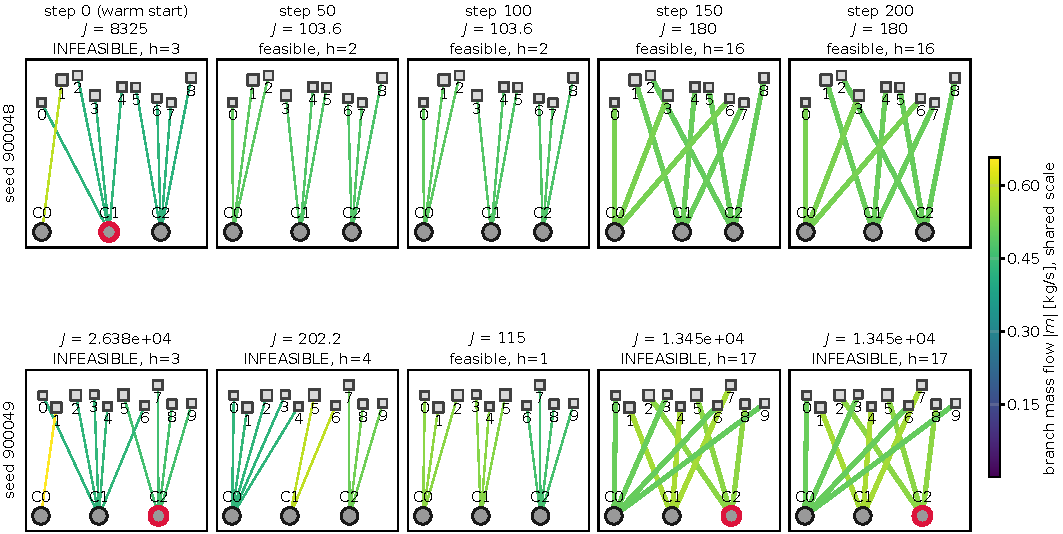
\includegraphics[width=\linewidth]{figures/design_trajectory.pdf}
\caption{One pathwise run at five checkpoints on four tasks: the design the agent emits while it
trains, with its deployed objective, feasibility and Hamming distance to the label.  Feasibility
arrives by step 50 on three of four tasks and is lost again by step 200 on two of them, while the
distance to the label grows from 2--5 decisions to 9--17.  No row is best at its endpoint: the visual form of this subsection's quantitative claim.}
\label{fig:traj}\end{figure*}
\cref{fig:traj} draws one run at five checkpoints before any of it is aggregated.
\section{Break-even controls: a search, a prompt and small policies}
\label{supp:baselines}
Three controls bound every post-training result in this paper, and all three are
cheap to run, and they are reported here in full. All use Benchmark~A v2, identical task rows, and the identical
regret $(\Jobj-\Jobj^\star)/|\Jobj^\star|$ against the strengthened best-known
reference.  They are reported as the mean of per-seed true medians, exactly as the note of Table~I of the main text does.  Every ratio below is therefore formed within one statistic, and
the controls are directly comparable to Sec.~VII-D of the main text, at five seeds.

\emph{(a) A search, with no model at all.}  Gradient-free full-neighbourhood
steepest descent reaches median regret $0.0673$ at feasibility $0.94$ on validation,
$0.2452$
% NOTE: case/policy/inference_search reports 0.0000 for its `steepest_full` arm on the
% same split.  The two are not in conflict and the difference is the stopping rule, not
% the method: inference_search runs to convergence (median 127 forward solves), while
% this arm is capped at --budget 400 with --stall 3 and shares that budget with the
% other arms of the comparison, and on the ood split it needs 312.  Quote 0.0000 when
% the claim is about what search achieves, and 0.0673 when the claim is about what it
% achieves at a matched budget.
at $0.75$ on test and $0.2234$ at $0.62$ out of distribution.  It consumes a median
of $186$ physics evaluations per task (range $30$--$421$). The range exceeds the nominal
$400$-evaluation cap on $9$ of $40$ tasks.  The cap is tested before a round rather
than during one, and a round at $N{=}16$ costs more than the remaining budget.  The comparison is therefore budget-matched to within
one round, not exactly, and is reported that way. Since the oracle that \emph{defines} regret is itself a
search, this is close to the ceiling, and no post-training claim can be a
single-task-quality claim. The defensible claim is amortisation.  Against the same
converged steepest-descent arm of the search case, the measured break-even is
$\sim910$ tasks by
wall clock and $\sim13$ by physics budget.  Both axes are built from the same named
comparator and the same mean statistic.  The budget-capped arm quoted in (a) would
move those to about $3{,}180$ tasks and about $8$ solves, so the break-even is a
property of the comparator, not of the method.  The two differ by two
orders of magnitude because a Benchmark~A solve costs $7$\,ms.  That is precisely the
regime in which the method is unnecessary.

\emph{(b) The same gradient information, as text.} The Introduction's claim that
handing the agent adjoint sensitivities in the prompt wastes information is measured here, and the claim is too strong as written. Injection is not ignored: relative to a plain prompt it improves the warm start
$5.0\times$ on validation ($1.0842\to0.2175$) and $25\times$ out of distribution
($7.4738\to0.2976$).  The model adopts the top-ranked suggested edit in $34$--$86\%$
of rounds on the warm start (per-task follow rate $0.340$--$0.859$) and
$34$--$100\%$ on the frozen base ($0.338$--$1.000$).  It is nonetheless dominated on every split by (a), by $3.2\times$ on validation and
$17\times$ on test.  The feasibility gap is the sharpest part: no single text arm
exceeds $0.50$ on validation, $0.38$ on test or $0.50$ out of distribution, against
$0.94/0.75/0.62$ for the search.  The best text arm also differs by split
($\texttt{steepest\_text}$ at $0.50$ on validation, $\texttt{sens\_exact}$ at $0.50$
out of distribution).  No text arm attains that triple simultaneously. The mechanism is measured rather than assumed.  The search changes exactly $1.00$
decision slots per round, which is all a single-edit linearisation licenses.  The
model changes $0.96$--$3.26$ slots per round on the warm start and $1.00$--$4.80$ on
the frozen base. It applies
the suggested edit \emph{and simultaneously rewrites several others}, and the
injected deltas are first-order in one coordinate at a time with no interaction
terms. Those ranges contain a counterexample to the mechanism as stated.
$\texttt{steepest\_text}$ changes $0.9604$ slots per round on validation and $0.9844$
on test: one edit at a time, exactly what the linearisation licenses.  It still loses
to the search ($0.2175$ against $0.0673$ on validation).  Run to convergence rather
than under the shared budget, the same search reaches median regret $0.0$; the two
search numbers differ only in the stopping rule. Edit discipline is therefore
necessary but not sufficient. Where the model is most disciplined is exactly where the text arms do best.
The information is therefore wasted not because the model cannot read it but
because a text prompt cannot make the \emph{accepted} design the one the linearisation
ranked.  That is a property of the interface, not of the base model.  A better base
model will not fix it. More text is worse, not better: the arm handed the
\emph{entire} simulated neighbourhood loses to the arm handed only the top six edits,
by $28\times$ out of distribution on the frozen base.
% source: ddl/case/llm/E5_prompt_sensitivity/loggers/20260914T204845Z_warmstart and
%         20260914T204845Z_frozenbase, --rounds 30 --G 4 --budget 400 --k 6.
%         follow_rate and hamming_prev per task in results_e5_prompt_sensitivity.json

\emph{The same adjoint as a twelve-solve greedy.}  Ranking the full
neighbourhood by the exact adjoint's first-order prediction and taking its best edit
reaches regret $0.153$ / $0.097$ / $0.076$ at feasibility $0.69$ / $0.63$ / $0.75$ for twelve physics solves. An alternating master/subproblem decomposition reaches
$0.0242$ / $0.0169$ / $0.0385$ for $514$--$1{,}111$ solves.  Both beat every learned
designer in this paper on design quality.  The defensible claim for post-training is
therefore amortisation and measurement, not single-task design.
% source: ddl/case/policy/greedy_and_oracle and ddl/case/policy/inference_search
%         (adjoint-greedy and decomposition arms); details in Supplementary Sec. S-II.

Controls (c) and (d) replace the language model with small policies and are
reported in Supplementary Sec.~S-II.  A 6{,}599-parameter factorised policy reaches
regret $15.73$ / $9.47$ / $7.86$ at five seeds: $169\times$ / $298\times$ /
$349\times$ better than an \emph{untransformed} score-function control that
diverges at this learning rate (Supplementary Sec.~S-II). It is $14.5\times$ worse
than the 4B warm start on validation.  Within a single pinned invocation, a
16{,}260-parameter graph policy beats the factorised policy by $5.92\times$ /
$8.41\times$ / $6.20\times$.  It wins feasibility on validation and test (exact McNemar $p=0.00031$ / $0.00091$; exact paired Wilcoxon on regret $p=0.0035$ /
$8.0\times10^{-5}$ / $0.014$).  The mechanism therefore does not require a language
model; what requires one is Supplementary Sec.~S-III.

Whether the agent can honour a constraint stated in English is measured in
Supplementary Sec.~S-III, and it is the only question on which a language model is
the sole candidate. A factorised policy cannot express ``racks R1 and R2 share a
CDU'' without retraining. An unconstrained search cannot express it at all.
The untrained base model satisfies held-out two-constraint draws significantly
better than any interface that cannot read them ($+0.542$ at $p=0.0003$ on
validation and $+0.375$ at $p=0.0042$ on test, against the factorised policy). Out of distribution the verdict is comparator-dependent ($p=0.064$ against
the policy, significant against the search).  Imitation training costs $25$ points
of compliance and removes the significance on both held-out splits.

The five-checkpoint plate of one run is \cref{fig:traj} of this supplement; the census of Supplementary Sec.~S-VII aggregates it.

\emph{(d) A learned surrogate of the solver.}  A per-task MLP (two 64-unit tanh
layers on the one-hot design vector, trained on the log of the hard-compile
objective).  Inside each cell it is trained on $400$ or $1{,}000$ random one-hot designs
and descended with its own gradient for $200$ normalised steps under the same race
protocol as (a) \cite{shahriari2016bayes,jones1998ego,brunton2020ml}.  At five seeds $\times$ five tasks per $N$: relaxed ratio
$0.204\pm0.144$ (sd, \texttt{ddof}=1) / $0.267\pm0.128$ (surr400) and $0.206\pm0.137$ / $0.229\pm0.105$
(surr1000), against $0.124\pm0.043$ / $0.164\pm0.032$ (pathwise) and
$0.236\pm0.070$ / $0.420\pm0.051$ (score-function).  The deployed hard objective is
$1{,}187\pm1{,}410$ / $3{,}032\pm2{,}364$ (surr1000) against $112\pm268$ /
$366\pm590$ (pathwise); held-out relative error $0.58$ / $0.47$ (median $0.62$ /
$0.44$).  Paired exact signed-rank over the $25$ (seed, task) cells per $N$:
surr1000 against pathwise $p=0.012$ / $0.0088$, surr400 against pathwise
$p=0.037$ / $4.5\times10^{-5}$, surr1000 against score-function $p=0.113$ /
$1.2\times10^{-7}$ (method exact\_dp).  The surrogate is directionally useful and
not shippable: its gradient descends the relaxed objective but its hard decodes are
an order of magnitude worse than the adjoint's.
% source: ddl/case/analysis/surrogate_baseline/loggers/20260916T021844Z_gpuserver/
%         results_surrogate.json -> rows[].{ste_t0.5,surr400,surr1000,reinforce}.
%         {relax,deployed}, rows[].surr1000.surr_rel_err; paired tests recomputed with
%         ddl/tools/summarize_runs.py:wilcoxon_signed_rank (exact_dp).

\section{The endpoint of a post-training run is not a stable summary of its recipe}
\label{supp:bstab}
Every table of post-training results in this paper reports a final value, and this section measures what
that convention costs.  Group all $60$ archived run directories on both benchmarks;
$40$ of them carry two or more checkpoints.  Group them by every argument in their
configuration except the run directory, the seed and the start time.  Comparing
realisations at matched evaluation steps then gives two spreads.  They must not
be conflated.  One is the spread \emph{within} a run across its own checkpoints.  The
other is the spread \emph{between} runs of one configuration.

\emph{Within a run.}  Across the $40$ measured runs the endpoint is the best
checkpoint in $8$, and in $3$ of the $27$ runs that carry a done row.  The worst
endpoint on record is $1{,}188\times$ the best checkpoint of its own run, a
Benchmark-B type-wise realisation that diverged mid-training.  Over the thirteen runs
of the two complete five-seed Benchmark-A score-function configurations (a third
group holds three realisations) the endpoint is best in $2$. Endpoint-over-best reaches $10.05$, and the median within-run worst-over-best
ratio over all measured runs is $7.126$.  \textbf{The final
checkpoint is the best one in $8$ of $40$ measured runs and the worst in $2$}.  One pathwise run on the production solver decodes to $109.18$, $452.97$,
$112.69$ and $185.89$ at checkpoints $0$, $50$, $100$ and $150$.  It is therefore
$4.1\times$ worse than its own warm start at step $50$ and within $3.2\%$ of it at
step $100$.

\emph{Between realisations of one configuration.} Two Benchmark-A score-function configurations have five
complete seeds each. At matched steps the decoded objective differs between seeds by up to
\textbf{$9.871\times$} in the first and \textbf{$12.57\times$} in the second, and the spread at the
endpoint is $9.871\times$ and $1.989\times$. On the production solver the same quantity reaches
$69.3\times$ between two seeds of the pathwise arm and $5.541\times$ between two runs of the
\emph{same seed on two different GPUs}, both complete. \textbf{The spread at step $0$ is exactly $1\times$
in every group}, so the divergence is generated by training rather than by initialisation.

\emph{Three consequences for how such a result may be reported.} First, quoting the endpoint understates:
the complete five-seed configurations end up to $10.05\times$ above their own best checkpoint. Second, quoting the best
checkpoint overstates, and is a nine-way maximum taken on the split being reported. Third, an
\emph{unpaired} comparison of two arms' endpoints has a resolution floor of roughly
$300\times$ at a matched step on Benchmark~B and $9.871\times$ between seeds of one
Benchmark-A configuration. This is why every arm comparison in this paper is a paired
per-task test, except the Sec.~VII-C race of the main text, which pairs per seed ($n=5$, the
finest granularity its artefact stores). It also explains why the graph-policy comparison of
\cref{supp:baselines} survives it: a paired Wilcoxon
conditions on seed and task instead of comparing endpoints.

\emph{What this does not say.} It does not say the instability belongs to one estimator.  At five
complete seeds the score-function arm is as unstable as the pathwise one, so no
arm-specific attribution of the instability is made.  The slot routing remains justified only by the bias
measurement, which is direct and unaffected. Nor does it say the recipe cannot be regularised.  A $20$-step single-seed probe of
it resolves no better than $4{,}544\times$, so no finer claim is made.
% source: ddl/case/analysis/run_stability/loggers/20260915T130706Z_gpuserver/
%         verdict.txt lines 45, 62, 109, 125 (combined census: 60 dirs, 40 measured,
%         best-in-8, worst 1,188x, median 7.126, 9.871x and 12.57x between-seed
%         spreads, ~300x unpaired floor); the two single-benchmark runs
%         20260915T091438Z and 20260915T084208Z are its inputs; results_run_stability.json ->
%         groups[].per_step[].max_over_min and runs[].within. The three trust-region cells are
%         ddl/case/llm/V5_warm_anchor/loggers/20260915T071704Z_gpuserver and
%         ddl/case/llm/V4_kl_anchor_probe/loggers/20260915T055837Z_gpuserver.
%         ddl/docs/RESULTS_index.md rows B17 and L13; ddl/docs/FINDINGS_2026-09-15.md s34-s37.
%         The GPU is not in args.json, so the same-seed two-GPU pair is identified from launch records.

\FloatBarrier

\section{Positioning table and post-training step}
\label{supp:position}
% Full-width float: the table gained two columns relative to the draft's Table I.
\begin{table*}[!t]\centering
\caption{Positioning.  ``Adjoint to weights'' means the simulator's Jacobian
reaches the designer's parameters.  That contrasts with its output value reaching
them as a reward or as prompt text, or its sensitivity field reaching them as a
conditioning input.  ``Relaxation is physical'' means every point of the relaxed
design space is a system the solver can simulate.  ``Pathwise bias'' records what
the work establishes about the bias of a first-order/pathwise gradient estimator;
``measured by decision type'' is a measurement on one production solver, not a
bound or a correction}
\label{tab:position}
\footnotesize
\setlength{\tabcolsep}{5pt}
\begin{tabular}{@{}lccccl@{}}\toprule
 & discrete & LLM & adjoint & relaxation & \\
 & structure & designer & to weights & is physical & pathwise bias\\
\midrule
Score-function post-training \cite{shao2024grpo,scidesignbench2026}
  & \checkmark & \checkmark & -- & n/a & none used (unbiased)\\
STE through tokens \cite{grade2026,diffro2025}
  & \checkmark$^{\dagger}$ & \checkmark & -- & -- & variance reported only\\
Amortized discrete inference \cite{hu2023abs}
  & \checkmark & \checkmark & -- & n/a & n/a (no simulator)\\
Differentiable-sim.\ policy gradients \cite{suh2022diffsim,onoda2026ddcg,scheffler2026cfobg}
  & -- & -- & \checkmark & n/a & analysed, switched, corrected\\
Unbiased mixed gradients \cite{hpo2026}
  & \checkmark & -- & \checkmark & -- & unbiased pathwise/SF mixture\\
Physics-driven designers \cite{jiang2019glonet}
  & -- & -- & \checkmark & n/a & n/a (continuous output)\\
Sensitivity-conditioned TO \cite{topotransformer2026}
  & -- & -- & adjoint as \emph{input} & n/a & n/a (continuous output)\\
LLM design agents \cite{ma2024sga,phythesis2025,jadhav2026mechdesigner}
  & \checkmark & \checkmark & -- & -- & none (no gradient)\\
Adjoint pipe-network TO \cite{blommaert2020adjoint,wack2022energy,wack2023gap}
  & \checkmark & -- & \checkmark & \checkmark & n/a (no learning)\\
Penalised fluid TO (Brinkman) \cite{borrvall2003topology}
  & -- & -- & \checkmark & \checkmark & n/a (no learning)\\
Concurrent water-network adjoint \cite{mu2026gga}
  & -- & -- & \checkmark & n/a & continuous parameters, status frozen\\
Trajectory-scored design agents \cite{zhang2026leap}
  & \checkmark & \checkmark & -- & n/a & none (Bayesian reference)\\
Ground-structure TO \cite{dorn1964automatic,zegard2014grand3d,guest2004minimum}
  & \checkmark & -- & -- & \checkmark & n/a (no learning)\\
Topological derivative \cite{sokolowski1999topological}
  & \checkmark & -- & -- & n/a & structural sensitivity theory\\
Neural combinatorial optimisation \cite{vinyals2015pointer,bello2017neural,kwon2020pomo}
  & \checkmark & -- & -- & n/a & none used\\
Grammar-constrained decoding \cite{hokamp2017lexically,post2018fast,willard2023guided}
  & \checkmark & partial & -- & n/a & n/a\\
RL evaluation methodology \cite{agarwal2021precipice,henderson2018matters}
  & -- & -- & -- & n/a & reporting standard adopted here\\
Density-field TO (SIMP) \cite{bendsoe1989simp}
  & -- & -- & -- & No & n/a (continuous field)\\
\textbf{This work}
  & \checkmark & \checkmark & \checkmark & \checkmark & measured by decision type\\
\bottomrule
\multicolumn{6}{@{}l@{}}{\footnotesize$^{\dagger}$discrete text or codec tokens,
not structural design decisions.}
\end{tabular}
\end{table*}

The positioning table (\cref{tab:position}) and the post-training step the main text summarises are given in full below.

\begin{algorithm}[t]
\caption{One post-training step (pathwise)}
\label{alg:stepS}
\begin{algorithmic}[1]
\STATE sample $B$ tasks; for each, decode $G$ designs under the \ddl{} grammar (no grad)
\STATE simulate each hard design: $\Jobj_g$ (logging / GRPO advantage)
\STATE teacher-forced pass $\to$ restricted logits $\ell$ with grad; same pass with adapters disabled $\to$ $\ell^{\mathrm{base}}$
\STATE conditional Gumbel + straight-through $\to$ $y^{\mathrm{ste}}$; $\soft=\rho(y^{\mathrm{ste}})$
\STATE physics forward at $\soft$ (on the solver GPU), adjoint (implicit-function theorem, main text) $\to$ $d\Jobj/d\soft$
\STATE loss $=\frac{1}{BG}\sum\Jobj/s+\beta\,\mathrm{KL}(\ell\|\ell^{\mathrm{base}})+\lambda_r\mathcal L_{\mathrm{replay}}$; backward; clip; AdamW on LoRA
\end{algorithmic}
\end{algorithm}

\section{Additional figures and the decision-type split table}
\label{supp:extrafigs}
The main text cites these objects by their supplementary numbers; this section holds them so that the main text stays within its page ceiling.
% source: floats of this section render from ddl/case/llm/V2_4b_estimators/loggers/ (nine
%         arms), ddl/case/benchB/E1d_edit_ranking/loggers/20260915T150207Z_edit5seed,
%         ddl/case/benchB/E0f_closure_repair/loggers/20260915T201056Z_gpuserver and
%         ddl/case/analysis/v2A_table/loggers/20260915T175120Z_gpuserver.

\begin{figure}[t]\centering
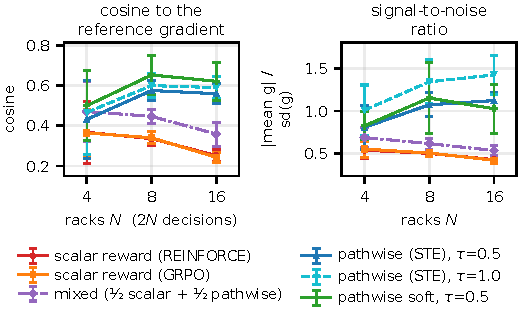
\includegraphics[width=\columnwidth]{figures/fig_e1c_estimators.pdf}
\caption{Gradient-estimator quality versus the number of design decisions on
Benchmark A (mean $\pm$ sd over 5 tasks $\times$ 2 policy points; $S{=}8$
physics evaluations per estimate; reference gradient from 2048 score-function
samples).  Cosine is taken to the reference gradient of the expected objective;
SNR is the norm of the mean estimate over the trace of its covariance.}
\label{fig:e1c}\end{figure}

\begin{figure}[t]\centering
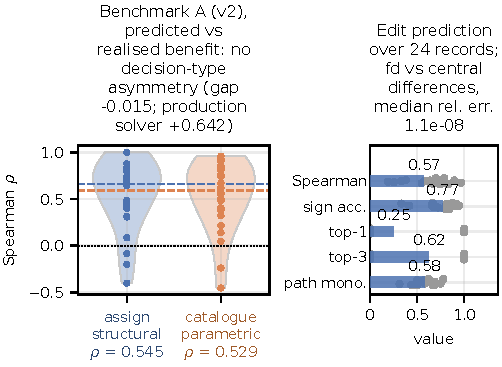
\includegraphics[width=\columnwidth]{figures/fig_e0_edits.pdf}
\caption{Left: per-design Spearman correlation between the first-order
pathwise prediction and the true benefit of every single structural edit (24
checks: six task seeds times four configurations, $N\in\{4,6,8\}$). Right:
aggregate sign accuracy, top-$k$ hit rates and fraction of edits whose objective is
monotone along the relaxation path.}
\label{fig:e0}\end{figure}

\begin{figure}[t]\centering
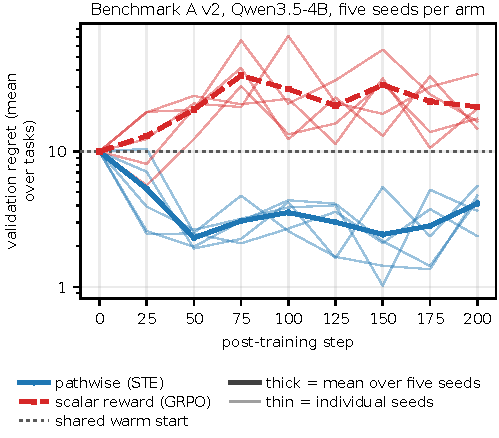
\includegraphics[width=\columnwidth]{figures/fig_e2_v2.pdf}
\caption{Validation regret against post-training step, five
seeds per arm.  Thick lines are the means over five seeds; thin lines are the
individual seeds; the dotted line is the shared warm start.}
\label{fig:e2}\end{figure}

\begin{figure}[t]
\centering
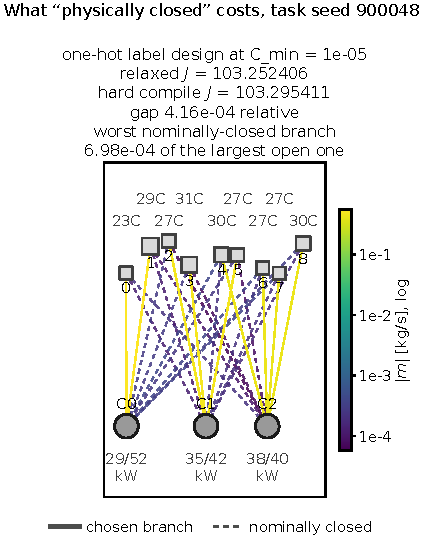
\includegraphics[width=0.86\linewidth]{figures/fig_lc_closure.pdf}
\caption{What ``physically closed'' costs, on one task.  The one-hot label design
evaluated as a \emph{soft} network at $C_{\min}=10^{-5}$ keeps every candidate branch
present with weight at least $C_{\min}$.  The branches a hard network would delete
still carry flow, drawn dashed and coloured on a log scale.  The largest
nominally-closed branch carries $6.98\times10^{-4}$ of the largest open one, and the
relaxed objective differs from the hard compile of the same design by
$4.16\times10^{-4}$ relative.  Both are instances of the floor in
\cref{tab:closure} of this supplementary, whose distance-sweep median at $C_{\min}=10^{-5}$ is
$6\times10^{-4}$.
}
\label{fig:lcclosure}
\end{figure}

\begin{table}[t]\centering\caption{Benchmark B: first-order prediction of a discrete
edit, split by decision type.  The two catalogue relaxations are within noise of each
other ($0.940$ vs $0.939$ rank correlation)}\label{tab:split}
\fontsize{7.2}{8.4}\selectfont
\begin{tabular}{@{}lccc@{}}\toprule
edit type & rank corr. & sign acc. & path monotone\\\midrule
assignment (structural) & $0.31$ & $0.66$ & $0.28$\\
catalogue (parametric) & $\mathbf{0.94}$ & $\mathbf{0.85}$ & $\mathbf{0.78}$\\
\bottomrule\end{tabular}\end{table}

\begin{figure}[t]\centering
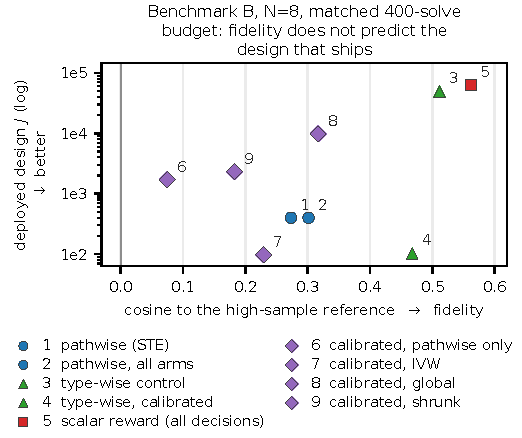
\includegraphics[width=\linewidth]{figures/fig_b_fidelity_vs_deployed}
\caption{The fidelity metric does not predict the design that ships.  Each point is
one estimator arm on Benchmark~B at $N{=}8$ under a matched $400$-evaluation budget:
cosine to a high-sample unbiased reference against the deployed objective of its
argmax-decoded design (log scale, lower better).  The best-aligned arm
($\cos=0.562$) ships $63501$; the pathwise arm ($\cos=0.273$) ships $400$,
$159\times$ better.  Shapes group estimator families; the artefact records nine
arms, eight with distinct deployed objectives.}
\label{fig:bfid}
\end{figure}

\begin{figure}[t]\centering
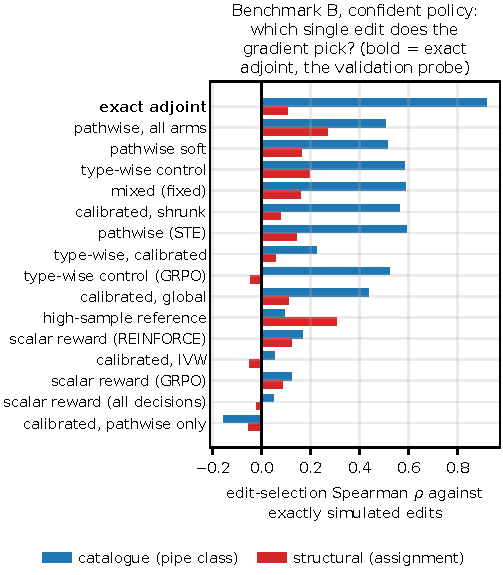
\includegraphics[width=\linewidth]{figures/fig_b_edit_ranking}
\caption{Edit selection at a confident policy point on Benchmark~B, split by
decision type: Spearman correlation between each arm's first-order prediction and the
exactly simulated edit effect, five seeds over ten policy points.  The exact adjoint
reaches $\rho=0.918$ on catalogue edits and $0.104$ on structural ones and picks the
true best edit in $8$ of $10$.  Every stochastic estimator degrades both, and the
scalar-reward arm is uncorrelated with the truth ($+0.0001$).}
\label{fig:bedit}
\end{figure}


\begin{table}[t]\centering\caption{Benchmark B: what the physical-closure floor costs, against a network in
which the unchosen branches are deleted.  Each median is over the five designs
feasible at that $C_{\min}$; the worst leak is the largest nominally-closed branch
flow over the largest open one.  No relaxed solve failed to converge in this sweep.  One hard compile per
$C_{\min}$ is rejected by the topology check: the same dead-end
design at all five floors, because the hard compile does not read $C_{\min}$.  The
pump column is not monotone in $C_{\min}$ ($0.11\%$ at $10^{-5}$ against $0.14\%$
at $10^{-6}$), so the floor is an order-of-magnitude statement.  The $C_{\min}$
column is the dimensionless length and minor-loss weight floor of the production
solver; on Benchmark A the same symbol denotes a conductance floor of
$2\times10^{-5}$\,kg$^2$\,s$^{-2}$\,kPa$^{-1}$}\label{tab:closure}
\fontsize{7.2}{8.4}\selectfont\setlength{\tabcolsep}{3pt}
\begin{tabular}{@{}lcccc@{}}\toprule
$C_{\min}$ & pump power & $\max T_{\mathrm{out}}$ & CDU duty & worst leak\\\midrule
$10^{-2}$ & $3.88\%$ & $1.97$\,K & $19.50\%$ & $80.2\%$\\
$10^{-3}$ & $2.85\%$ & $1.57$\,K & $15.82\%$ & $33.4\%$\\
$10^{-4}$ & $1.00\%$ & $0.71$\,K & $7.11\%$ & $11.4\%$\\
$\mathbf{10^{-5}}$ & $\mathbf{0.11\%}$ & $\mathbf{0.048}$\,\textbf{K} & $\mathbf{1.00\%}$ & $2.15\%$\\
$10^{-6}$ & $0.14\%$ & $0.043$\,K & $0.10\%$ & $0.23\%$\\
\bottomrule\end{tabular}\end{table}

\section{Benchmark-A physicality audit and repair}
\label{supp:audit}
The first physics configuration of Benchmark A admitted non-physical designs that
its own labels made computable.  Enumerating every design of the enumerable sizes
under the legacy configuration gives $13{,}122$ solves with an objective dynamic
range of $1.40\times10^{10}$.  Of these, $414$ designs carry negative rack or pump
flow ($881$ negative rack flows, $403$ negative pump flows).  Under the repaired
configuration (check-valve pump model, $100$\,K temperature cap) the same
enumeration gives a dynamic range of $4.05\times10^{4}$ and $6$ non-physical
designs.  The range reduction is $3.46\times10^{5}$, and the adjoint of the
repaired solver remains exact against central differences.  Sampled designs under
the legacy configuration show a dynamic range of only $1.18\times10^{3}$, which is
why sampling-based checks missed the failure.  The repair is verified against
enumeration wherever enumeration is possible.  On the $12$ of $40$ evaluation rows
small enough to enumerate completely, the best-known reference equals the true
optimum exactly (median, mean, maximum and minimum alike, non-negative fraction
$1.0$).
% source: ddl/case/benchA/E0a_physicality_audit/loggers/20260914T183018Z_gpuserver/
%         results_e0a.json -> enumerated.{legacy|raw, checkvalve|tempered}.
%         {J_dynamic_range, designs_with_neg_flow, neg_rack_flow, neg_pump_flow},
%         sampled["legacy|raw"].J_dynamic_range, verdict.{dynamic_range_reduction,
%         adjoint_still_exact}; enumeration verification from
%         ddl/case/policy/greedy_and_oracle/loggers/20260915T092629Z_gpuserver/
%         results_greedy_oracle.json -> reference_slack.
\section{Benchmark-B post-training: full tables and tests}
\label{supp:e2B}
\subsection{Post-training on the production solver}
\label{sec:e2B}
On Benchmark~B the same recipe trains against the production solver at $48$
training rows against Benchmark A's $64$.  Pathwise and GRPO carry five seeds at
step 200; the type-wise control carries four: its fifth run died at step 178 to a
CUDA device-side assert, is re-running, and nothing here imputes it.  At five seeds
the production solver supplies the paper's sharpest negative: every arm regresses
against its own warm start on regret.  Pathwise is worse on every split in the
pooled per-(seed, task) rows ($p=0.0045$ / $0.00075$ / $0.012$) and inseparable on
the seed-mean primary ($p=0.12$ / $0.18$ / $0.38$).  GRPO is worse on
validation and test on seed-mean ($p=0.034$ / $0.034$), and the type-wise control
diverges ($5.1\times10^{5}$ / $3.2\times10^{5}$ / $879$ against the warm start's
$28$ / $44$ / $69$; seed-mean $p=0.00015$ / $0.0021$ / $0.023$).  Feasibility moves
little and not significantly: pathwise $0.700$ / $0.825$ / $0.650$ against the warm
start's $0.688$ / $0.750$ / $0.625$ (Fisher $p=1$ / $0.49$ / $1$).  A Holm adjustment
over the eighteen seed-mean tests retains five, all of them comparisons against the
diverging type-wise arm.  They are type-wise against the warm start on validation and test,
pathwise against type-wise on validation and test, and GRPO against type-wise on
validation.  Endpoints are not benign either: endpoint-over-best reaches $23$ for
pathwise and $6.4\times10^{5}$ for type-wise (medians $1.47$ / $1.69$ / $37.4$ over
15/15/12 runs).  On the solver where amortisation was supposed to bite,
post-training at 200 steps regresses against imitation training.
% source: ddl/case/analysis/v2B_table/loggers/20260916T033403Z_gpuserver/
%         results_v2B_table.json -> table, paired_wilcoxon (pooled and seed-mean,
%         exact_dp), Fisher counts, endpoint census; type-wise at four seeds with the
%         fifth re-running after a CUDA device-side assert at step 178.
% source: ddl/case/analysis/round10_reanalysis/loggers/20260916T033647Z_gpuserver/
%         results_round10.json -> sec3_holm.benchmark_B.holm_seedmean (5 of 18).
Pooled per-(seed, task) rows give pathwise against the warm start $p=0.0045$ /
$0.00075$ / $0.012$, type-wise against the warm start $p=0.010$ / $7.4\times10^{-5}$
/ $0.0035$, and GRPO against the warm start $p=0.14$ / $0.0019$ / $0.91$.  Pathwise
against type-wise gives $p=0.28$ / $0.00011$ / $0.043$; GRPO against type-wise
$p=0.0031$ / $8.4\times10^{-6}$ / $0.0056$; pathwise against GRPO $p=0.30$ / $0.23$
/ $0.19$.  Feasibility counts: pathwise 56/80, 66/80, 26/40; GRPO 49/80, 45/80,
26/40; type-wise 30/64, 27/64, 16/32; warm start 11/16, 12/16, 5/8.


\begin{figure*}[!t]\centering
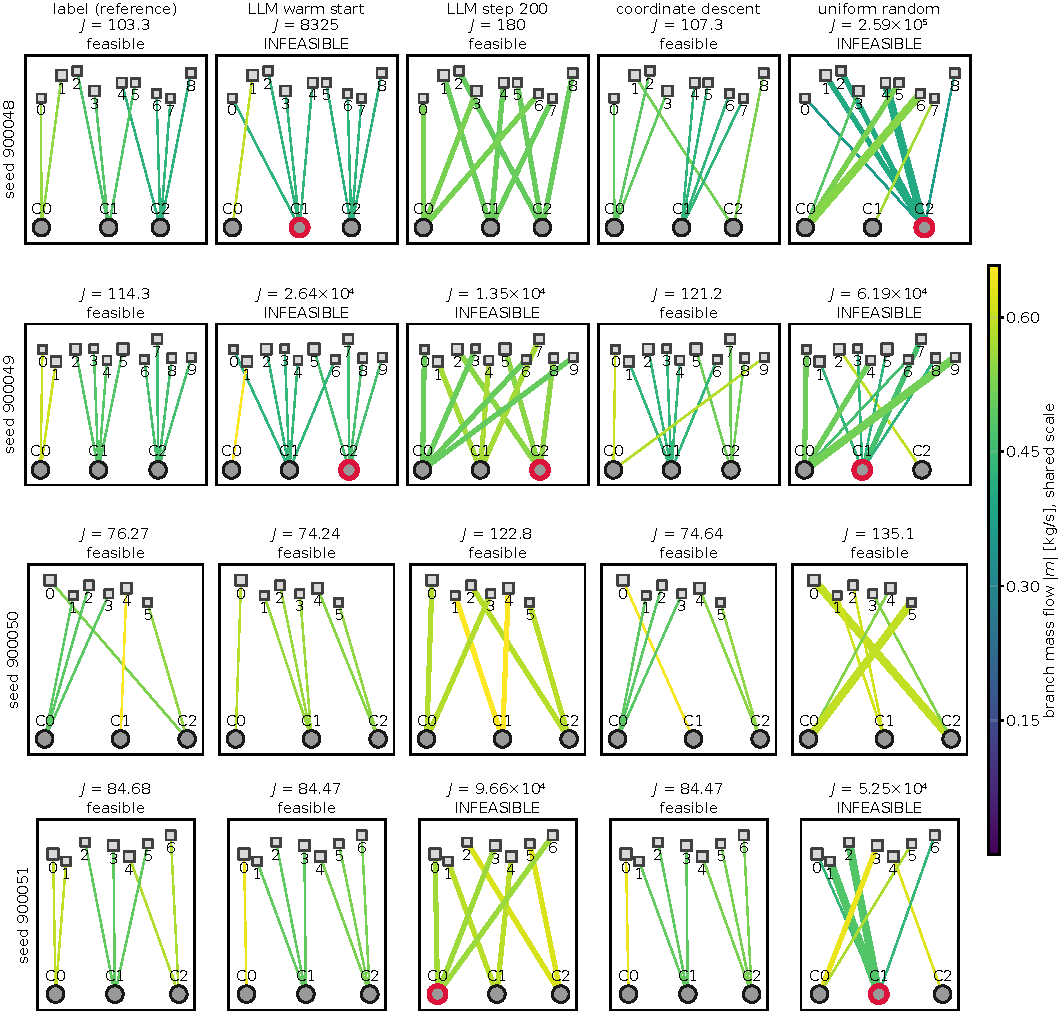
\includegraphics[width=\linewidth]{figures/case_gallery.pdf}
\caption{What each method designs on two Benchmark-B validation tasks (seeds
900048 and 900049); the four-task plate is in the companion repository.  Panels
draw racks (squares, area by heat load) and CDUs (circles); pipe colour and width
are the solved mass flow and the chosen diameter class, and a crimson ring marks
each violated constraint.  The language model was warm-started and post-trained on
Benchmark~B and decoded here unchanged.  Its step-200 design is feasible on one of
these two tasks and never beats two seconds of coordinate descent on either; the
uniform draw is infeasible on both, violating CDU capacity on both.}
\label{fig:galleryS}\end{figure*}

\begin{table*}[t]\centering\caption{Arm-by-criterion matrix on Benchmark~B: gradient-estimate alignment, relaxed descent, shipped design and discrete edit selection at the confident policy point, per estimator arm}
\label{tab:armmatrix}
\footnotesize\setlength{\tabcolsep}{4pt}
\begin{tabular}{l cc cc cc cc}
\toprule
arm & $\cos$ N8 & $\cos$ N16 & relax N8 & relax N16 & deploy N8 & deploy N16 & edit $\rho$ & top-1 \\
\midrule
pathwise (straight-through) & 0.27 & 0.25 & 0.417 & 0.642 & 400 & 397 & 0.477 & 0.80 \\
all-pathwise & 0.30 & 0.29 & 0.417 & 0.642 & 400 & 397 & 0.451 & 0.40 \\
score-function & 0.56 & 0.27 & 0.872 & 0.951 & 63501 & 240837 & 0.000 & 0.20 \\
type-wise & 0.51 & 0.37 & 0.730 & 0.884 & 49334 & 77299 & -- & -- \\
calibrated, global & 0.32 & 0.05 & 0.454 & 0.804 & 9791 & 344 & 0.302 & 0.00 \\
calibrated, shrunk & 0.18 & 0.23 & 0.511 & 0.665 & 2316 & 631 & 0.401 & 0.10 \\
calibrated, IVW & 0.23 & 0.18 & 0.777 & 1.040 & 97 & 103757 & 0.137 & 0.00 \\
soft-forward & -- & -- & -- & -- & -- & -- & 0.448 & 0.10 \\
REINFORCE & -- & -- & -- & -- & -- & -- & 0.156 & 0.10 \\
GRPO & -- & -- & -- & -- & -- & -- & 0.095 & 0.00 \\
\bottomrule
\end{tabular}
\par\medskip
{\footnotesize Cosine is to the reference gradient of the relaxed objective ($n=10$ per cell).  Relaxed descent is final/start relaxed objective, and shipped design the hard-compile objective of the greedy decode, both means over five seeds.  Edit selection is Spearman and top-1 over ten policy points.  Dashes mark criteria an arm was not measured on.  The edit-selection entry of the pathwise row is the deterministic exact-adjoint probe, not the straight-through estimator; the pathwise and all-pathwise rows coincide bitwise on the shipped design.\par}
% source: ddl/case/benchB/E1b_estimator_types/loggers/20260915T150205Z_race5seed_calibbugfix/
%         results_e1b_lc.json -> summary.stats (cos_of_mean, n=10), summary.race (relaxed
%         mean/sd, n=5), race[].greedy[-1][1] (deployed, n=5); edit columns from
%         ddl/case/benchB/E1d_edit_ranking/loggers/20260915T150207Z_edit5seed/
%         results_e1d_edit_ranking.json -> summary[confident|*].
\end{table*}

\section{Solver non-convergence under relaxation: counts, rescues and exceptions}
\label{sec:sxii}
\emph{An engineering observation.}  Relaxing a production solver exposes numerical behaviour that its own design
space never reaches.  The GGA's Newton step fails to converge on a minority of
relaxed designs, entering a non-converging oscillation of the undamped step
near the laminar--turbulent blend.  The failure is not the Jacobian clamp, which floors the conductivity gradient
at $10^{-8}$\,Pa\,s/kg, four orders below the smallest conductivity iterate entry observed.  In the
closure sweep all $90$ relaxed solves converged under the deployed damped Newton
with backtracking and continuation.  The five
failures at $5.6\%$ are hard compiles of a single dead-end design, rejected by the
topology check identically at all five $C_{\min}$ because the hard compile does not
read $C_{\min}$.  The archived rescue counters give the undamped-failure rate where it exists. In the edit-ranking solves of the same run, the archived cumulative counters are
$179$ damped-Newton rescues and $16$ continuation rescues; no per-solve
denominator is archived, so no rate is quoted.
The failures localise in \emph{design} space rather than in $C_{\min}$.  Over
$12{,}800$ relaxed solves drawn at a controlled distance $\varepsilon$ from the
label design, $0$ of $5{,}120$ fail at $\varepsilon<0.1$ and $10$ of $7{,}680$
($0.13\%$) fail at $\varepsilon\ge0.1$.  It never fails at the label design or within
half a decision of it and starts failing once designs are one decision away, which is
part of the regime a post-training run explores.  The three
Benchmark-B arms that completed $200$ steps drew $6{,}400$, $3{,}200$ and $6{,}400$
relaxed solves and recorded \emph{zero} crashes.  A failed sample is not fatal in
any case: the estimator replaces it with the detached mean of the samples that
converged, and returns a zero-gradient step when a whole group fails.  So the honest statement is that non-convergence is rare, and that it is
concentrated beyond one decision from a good design.  The curve says where it lives.
It does not say that a long run must crash: the same paragraph's $0$-of-$5{,}120$
contradicts the stronger claim.
% source: case/analysis/sampling_tail_control/loggers/20260915T051016Z_gpuserver/
%         results_sampling_tail.json -> results[bench=B].relaxed_solver.{n_failed_solves,n_solves};
%         ddl/docs/FINDINGS_2026-09-15.md s30.3. Failure handling follows the trainer's own rule
%         (ste.pathwise_objective substitutes the detached mean of the converged samples).
The solver runs
damped Newton with backtracking and continuation always on and exposes no undamped
mode, so earlier multi-mode ladders were never configurations of a single
measurement.
A genuine three-mode ladder
would require instrumentation flags inside the production solver module, which is
shared with
other work in this repository and was not modified for it.  We report this
at all because it is a cost of the method that a reader adopting it will pay.


\section{Benchmark-A paired-test census behind Table~I}
\label{supp:acensus}
The primary paired test of Table~I of the main text is the exact tie-aware
signed-rank test on one pair per task over the seed-mean regret ($n=16$/$16$/$8$).
Pathwise against GRPO gives $p=0.011$ / $9.2\times10^{-5}$ / $0.0078$; pathwise
against the warm start $p=0.71$ / $0.12$ / $0.0078$; GRPO against the warm start
$p=0.034$ / $0.0092$ / $0.31$.  Type-wise control against the warm start gives
$p=0.94$ / $0.50$ / $0.15$; against pathwise $p=0.27$ / $0.051$ / $0.023$; against
GRPO $p=0.025$ / $4.3\times10^{-4}$ / $0.0078$.  A Holm adjustment over these
eighteen tests retains two: pathwise against GRPO on test and GRPO against
type-wise on test.  The pooled per-(seed, task) convention ($n=80$/$80$/$40$) is
reported beside it as a sensitivity analysis only.  The warm start is one adapter
decoded identically by every seed, and the task axis clusters the cells (ICC up to
$0.95$, effective $n$ as low as $9$ of $40$).
% source: ddl/case/analysis/v2A_table/loggers/20260915T175120Z_gpuserver/
%         results_v2A_table.json -> paired_wilcoxon and paired_wilcoxon_seedmean
%         (wilcoxon_method exact_dp in every cell); Holm from
%         ddl/case/analysis/round10_reanalysis/loggers/20260916T033647Z_gpuserver/
%         results_round10.json -> sec3_holm.benchmark_A.


\FloatBarrier
\bibliographystyle{IEEEtran}
\ifblindreview\bibliography{references_blind}\else\bibliography{references}\fi
\end{document}
